\documentclass[letterpaper]{article}
	
\usepackage{fullpage}
\usepackage{mathtools}
\usepackage{qtree}
\usepackage[section]{placeins}
\usepackage{subcaption}
\usepackage{float}
\DeclarePairedDelimiter{\ceil}{\lceil}{\rceil}
\DeclarePairedDelimiter{\floor}{\lfloor}{\rfloor}
{\renewcommand{\arraystretch}{1.2}
\usepackage{wrapfig}
\usepackage{changepage}  
\usepackage{listings}
\usepackage{changepage}

\title{CS405G Final Project Report}

\author{Matt Ruffner, Mati Turner, Matt Dunbar\\ \small{github.com/ruffner/e-commerce}}

\begin{document}
\maketitle

%%%%%%%%%%%%%%%%%%%%%%%%%%%%%%%
%%%%%%%%%%%%%%%%%%%%%%%%%%%%%%% OUTLINE TAKEN FROM PROJECT SITE
%%%%%%%%%%%%%%%%%%%%%%%%%%%%%%%
\section{Finalized Database Design}

\subsection{Detailed ER diagram}
\begin{figure}[H]
\centering
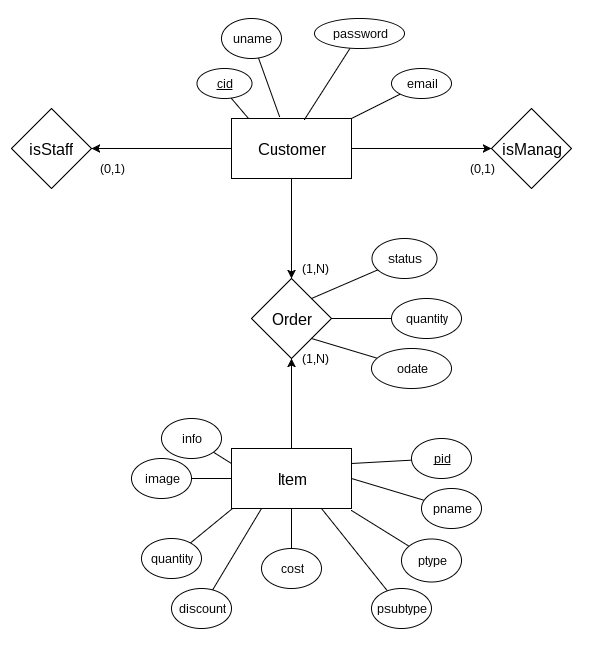
\includegraphics[width=\textwidth]{final-er}
\caption{Final ER Diagram}
\label{er}
\end{figure}
\subsection{Detailed database schema design}
For table definitions, our code: 

\begin{adjustwidth}{2cm}{0cm}
\begin{lstlisting}[language=sql]
CREATE TABLE Customer (
	cid INTEGER NOT NULL AUTO_INCREMENT,
	uname VARCHAR(100) NOT NULL,
	password VARCHAR(100) NOT NULL,
	email VARCHAR(100) NOT NULL,
	PRIMARY KEY(cid),
	CHECK (LEN(password) > 5)
) ENGINE=INNODB;

CREATE TABLE Staff (
	sid INTEGER NOT NULL,
	FOREIGN KEY(sid) REFERENCES Customer(cid)
) ENGINE=INNODB;

CREATE TABLE Manager (
	mid  INTEGER NOT NULL,
	FOREIGN KEY(mid) REFERENCES Customer(cid)
) ENGINE=INNODB;

CREATE TABLE Item (
	pid INTEGER NOT NULL AUTO_INCREMENT,
	pname VARCHAR(500) NOT NULL,
	ptype VARCHAR(100) NOT NULL,
	psubtype VARCHAR(100),
	cost REAL NOT NULL,
	discount REAL NOT NULL,
	quantity INTEGER NOT NULL,
	image VARCHAR(100),
	info VARCHAR(1000),
	PRIMARY KEY(pid),
	CHECK (cost > 0),
	CHECK (discount < 1 AND discount >=0),
	CHECK (quantity >=0)
) ENGINE=INNODB;

CREATE TABLE Orders (
	cid INTEGER NOT NULL,
	pid INTEGER NOT NULL,
	status VARCHAR(100) NOT NULL,
	quantity INTEGER NOT NULL,
	odate DATETIME,
	FOREIGN KEY(cid) REFERENCES Customer(cid),
	FOREIGN KEY(pid) REFERENCES Item(pid),
	CHECK (cid IN (SELECT cid FROM Customer)),
	CHECK (pid IN (SELECT pid FROM Item)),
	CHECK (status="cart"),
	CHECK (quantity > 0)
) ENGINE=INNODB;
\end{lstlisting}
\end{adjustwidth}

From the ER Diagram, it’s a pretty simple step to turn it into tables.  The manager and staff tables simply hold the mid and sid as references to the “customer” entity they stem from.  The order table contains the part and customer IDs that make up the relationship.  The customer and item entities translate directly into tables.  The status trigger in the orders table makes sure that upon creation, the item is listed in a cart because that is how the program flow dictates any entry should originate.

\subsection{Functional Dependencies}
Manager and staff tables are omitted from the relational dependency analysis below, for they’re really just customer tables.

\subsubsection{Customer}
Let $A=cid, B=uname, C=password, D=email.$ Then $A \rightarrow B, A \rightarrow C, A \rightarrow D$.  

From the key, all values can be determined, there are no dependencies on any non-key attribute.  Customer table is 3NF.

\subsubsection{Order}
Let $A=cid, B=pid, C=status, D=quantity$. Then $AB \rightarrow C, AB \rightarrow D, AB \rightarrow E$	

From the candidate key obtained by combining the cid and pid of the order, we can find the other members of the table.  There aren’t any dependencies within the row among the data members, thus each can be determined by the combination of the keys.  The Orders table is 3NF.



\subsubsection{Item}

Let $A=pid, B=pname, C=ptype, D=psubtype, E=cost, F=discount, G=image, H=info$. Then $A \rightarrow B, A \rightarrow C, AC \rightarrow D,  A \rightarrow E,  A \rightarrow F, A \rightarrow G, A \rightarrow H$.

Every model can be determined by the pid or the combination of the pid and type (in the case of subtype).  Thus there aren’t any non-trivial dependencies on anything other than the key or a superkey.  As such, the Item table is 3NF.




%%%%%%%%%%%%%%%%%%%%%%%%%%%%%%%%
%%%%%%%%%%%%%%%%%%%%%%%%%%%%%%% DESCRIPTION OF PROGRAMS
%%%%%%%%%%%%%%%%%%%%%%%%%%%%%%%%
\section{Description of programs}
\subsection{Program flow}

This web application is designed on an asynchronous model which preforms all data transfer via AJAX requests, eliminating the need for page reloads. The site is constructed using Google's material design web components, the PolymerElements.\cite{polymer} 

When a customer visits the site, a PHP session variable is populated which contains the database connection which may be queried upon subsequent requests. 

Various PHP pages were purpose written and separated by functionality. Templating and databinding, offered by Polymer, allow control over DOM visibility, making it easy to show 'admin' views only if the corresponding variable is set in the user structure/object. This may see like a vulnerability since the JavaScript object can be modified after pageload. This is not the case however, since all PHP pages which preform actions requested by admin views (order submitting, item updating/shipping, etc) first verify that the user requesting the actions does indeed have permission to. 

\subsection{Data structures}
The PHP array seen in Fig. \ref{user-struct} is stored in a \texttt{\$\_SESSION} variable, it holds user information and is passed back with every AJAX request to the front end. By specifying the header of the PHP page's output to be JSON, with \texttt{Content-Type: application/json}, arrays like the one seen in Fig. \ref{user-struct} are converted to JavaScript objects. To send the array below back to the front end, the PHP would be \texttt{echo json\_encode(\$BLANK\_USER)}. 

  The Iron Element \texttt{iron-ajax} is used to handle asynchronous requests. Dot notation is then used on the font end to access the information. An \texttt{iron-ajax} might be implemented as seen in Fig. \ref{ajax}. The \texttt{on-response} tag specifies a callback for the data to be passed to. To extract the users email address from the received data, assuming the signature \texttt{handleResponse(e)}, would then be \texttt{e.detail.response.email}
\begin{figure}[H]
\begin{adjustwidth}{.3\textwidth}{0cm}

\begin{lstlisting}[language=php]
$BLANK_USER = Array(
	"uname" => "",
	"email" => "",
	"isStaff" => False,
	"isManager" => False
);
\end{lstlisting}
\end{adjustwidth}
\caption{PHP structure to hold user information.}
\label{user-struct}
\end{figure}

\begin{figure}[H]
\begin{adjustwidth}{.3\textwidth}{0cm}

\begin{lstlisting}[language=html]
<iron-ajax
    url="../src/products.php"
    handle-as="json"
    on-response="handleResponse">
</iron-ajax>
\end{lstlisting}
\end{adjustwidth}
\caption{Example }
\label{ajax}
\end{figure}
\subsection{Algorithms}
One interesting portion of code is the JavaScript which processes the orders from the SQL table to be shown in the order cards for the user. An image of the order card can be seen in Fig. \ref{order-card} In the database, there is one row for each item in an order, with unique dates grouping items in the same order (\textit{odate} is NULL if the item is in the users cart). 
\begin{small}
\begin{lstlisting}[language=c++]
computeOrders: function(o) {
  var g = []; // to hold orders grouped by order date
        
  if(o && o.length ){ // if we have orders to show
    var time = '';
    var total = 0;
    
    // go through each order
    for( var i=0; i<o.length; i++ ){
    
      o[i].price = o[i].price * o[i].quantity;  // adjust price
      
      // if this is a new odate group
      if( time != o[i].odate ){
        // new order but not first,  assign total thusfar
        if(total)
          g[g.length-1].total = total;
        total = o[i].price;

        // push a new model, representing one order card each item in the items 
        // list gets iterated over by the inner template
        g.push({
          odate: o[i].odate, 
          cid: o[i].cid,
          items: [ o[i] ],
          status: o[i].status,
          statusMessage: "",
          pending: (o[i].status == "pending"),
          total: total,
          uname: o[i].uname,
          email: o[i].email
        });

        time = o[i].odate
      } 
      // an item from the same order 
      else {
        g[g.length-1].items.push( o[i] );  // add it to the most recent items array

        total += o[i].price; // add its price to the total

        if( i == o.length-1 ) // assign the last total since loop wont go again
          g[g.length-1].total = total;
      }
    }
    return g;
  } else {
    console.log("no orders to group");
  }
}
\end{lstlisting}
\end{small}


\section{Program functions}
\subsection{Sample input and output screens for each function}

\subsubsection{Login Screen}
\begin{figure}[H]
\centering
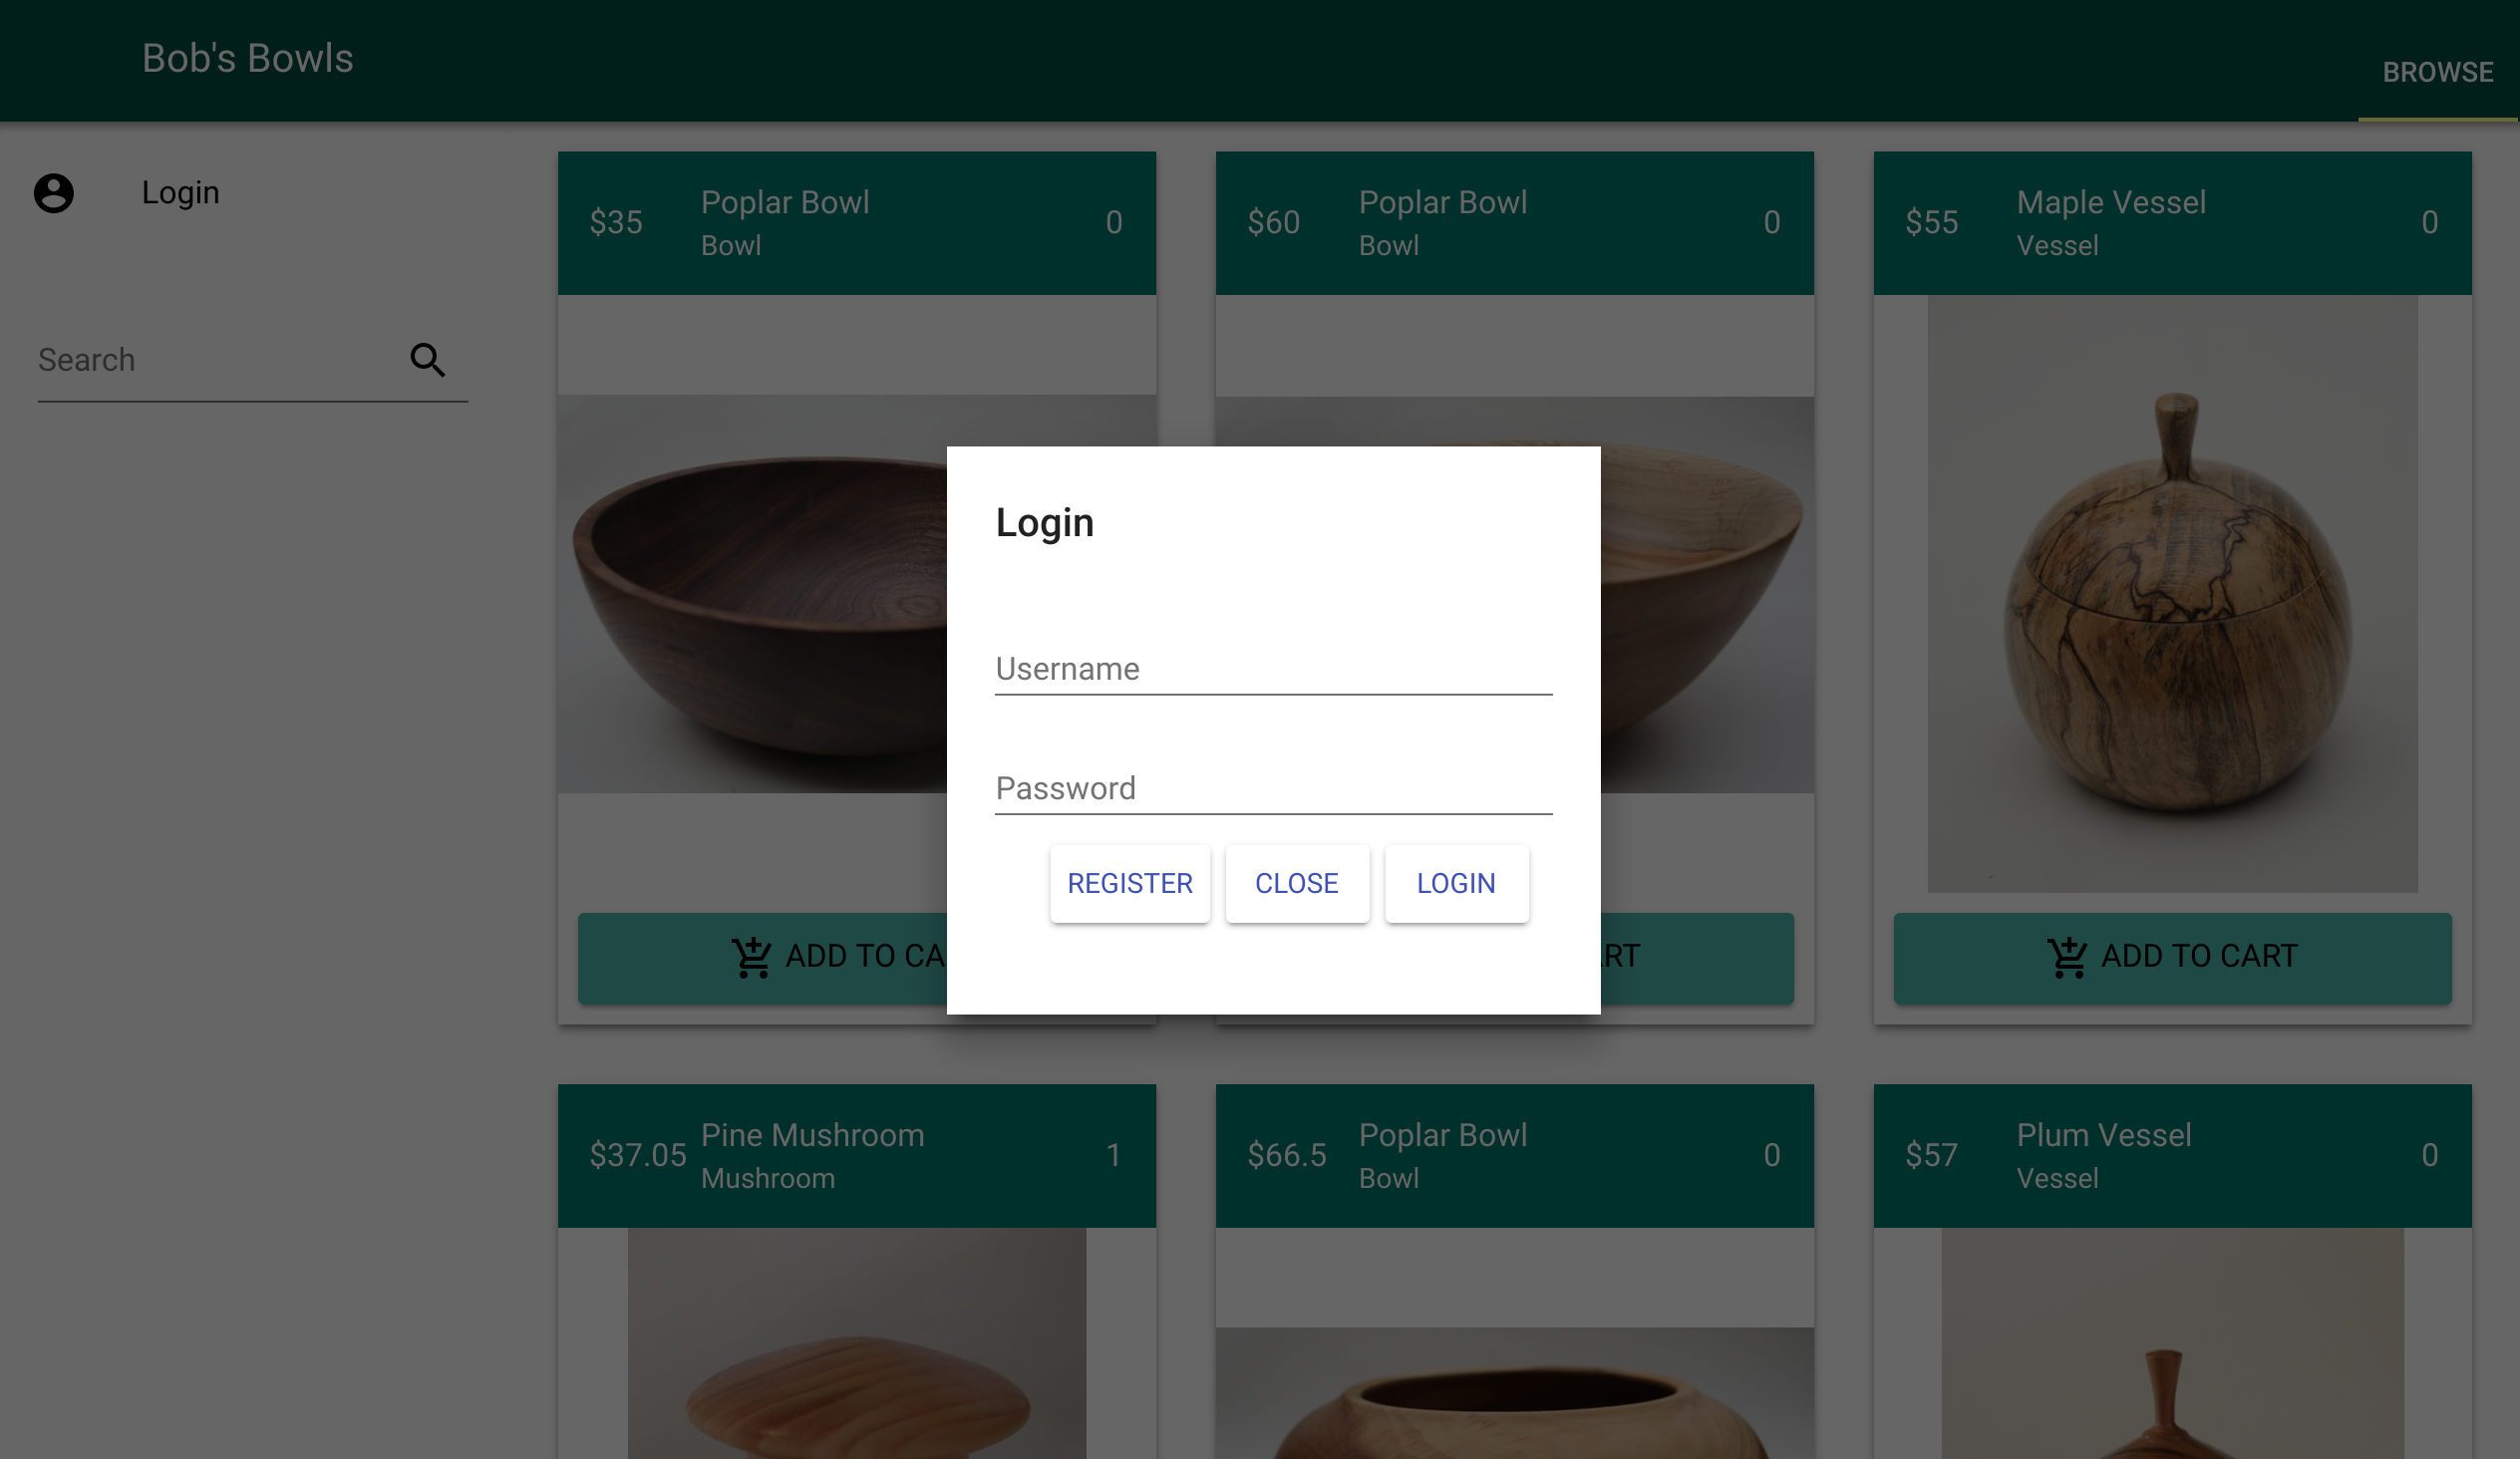
\includegraphics[width=.8\textwidth]{login}
\caption{The Login Screen}
\label{cap-login}
\end{figure}


\subsubsection{After User Login}
\begin{figure}[H]
\centering
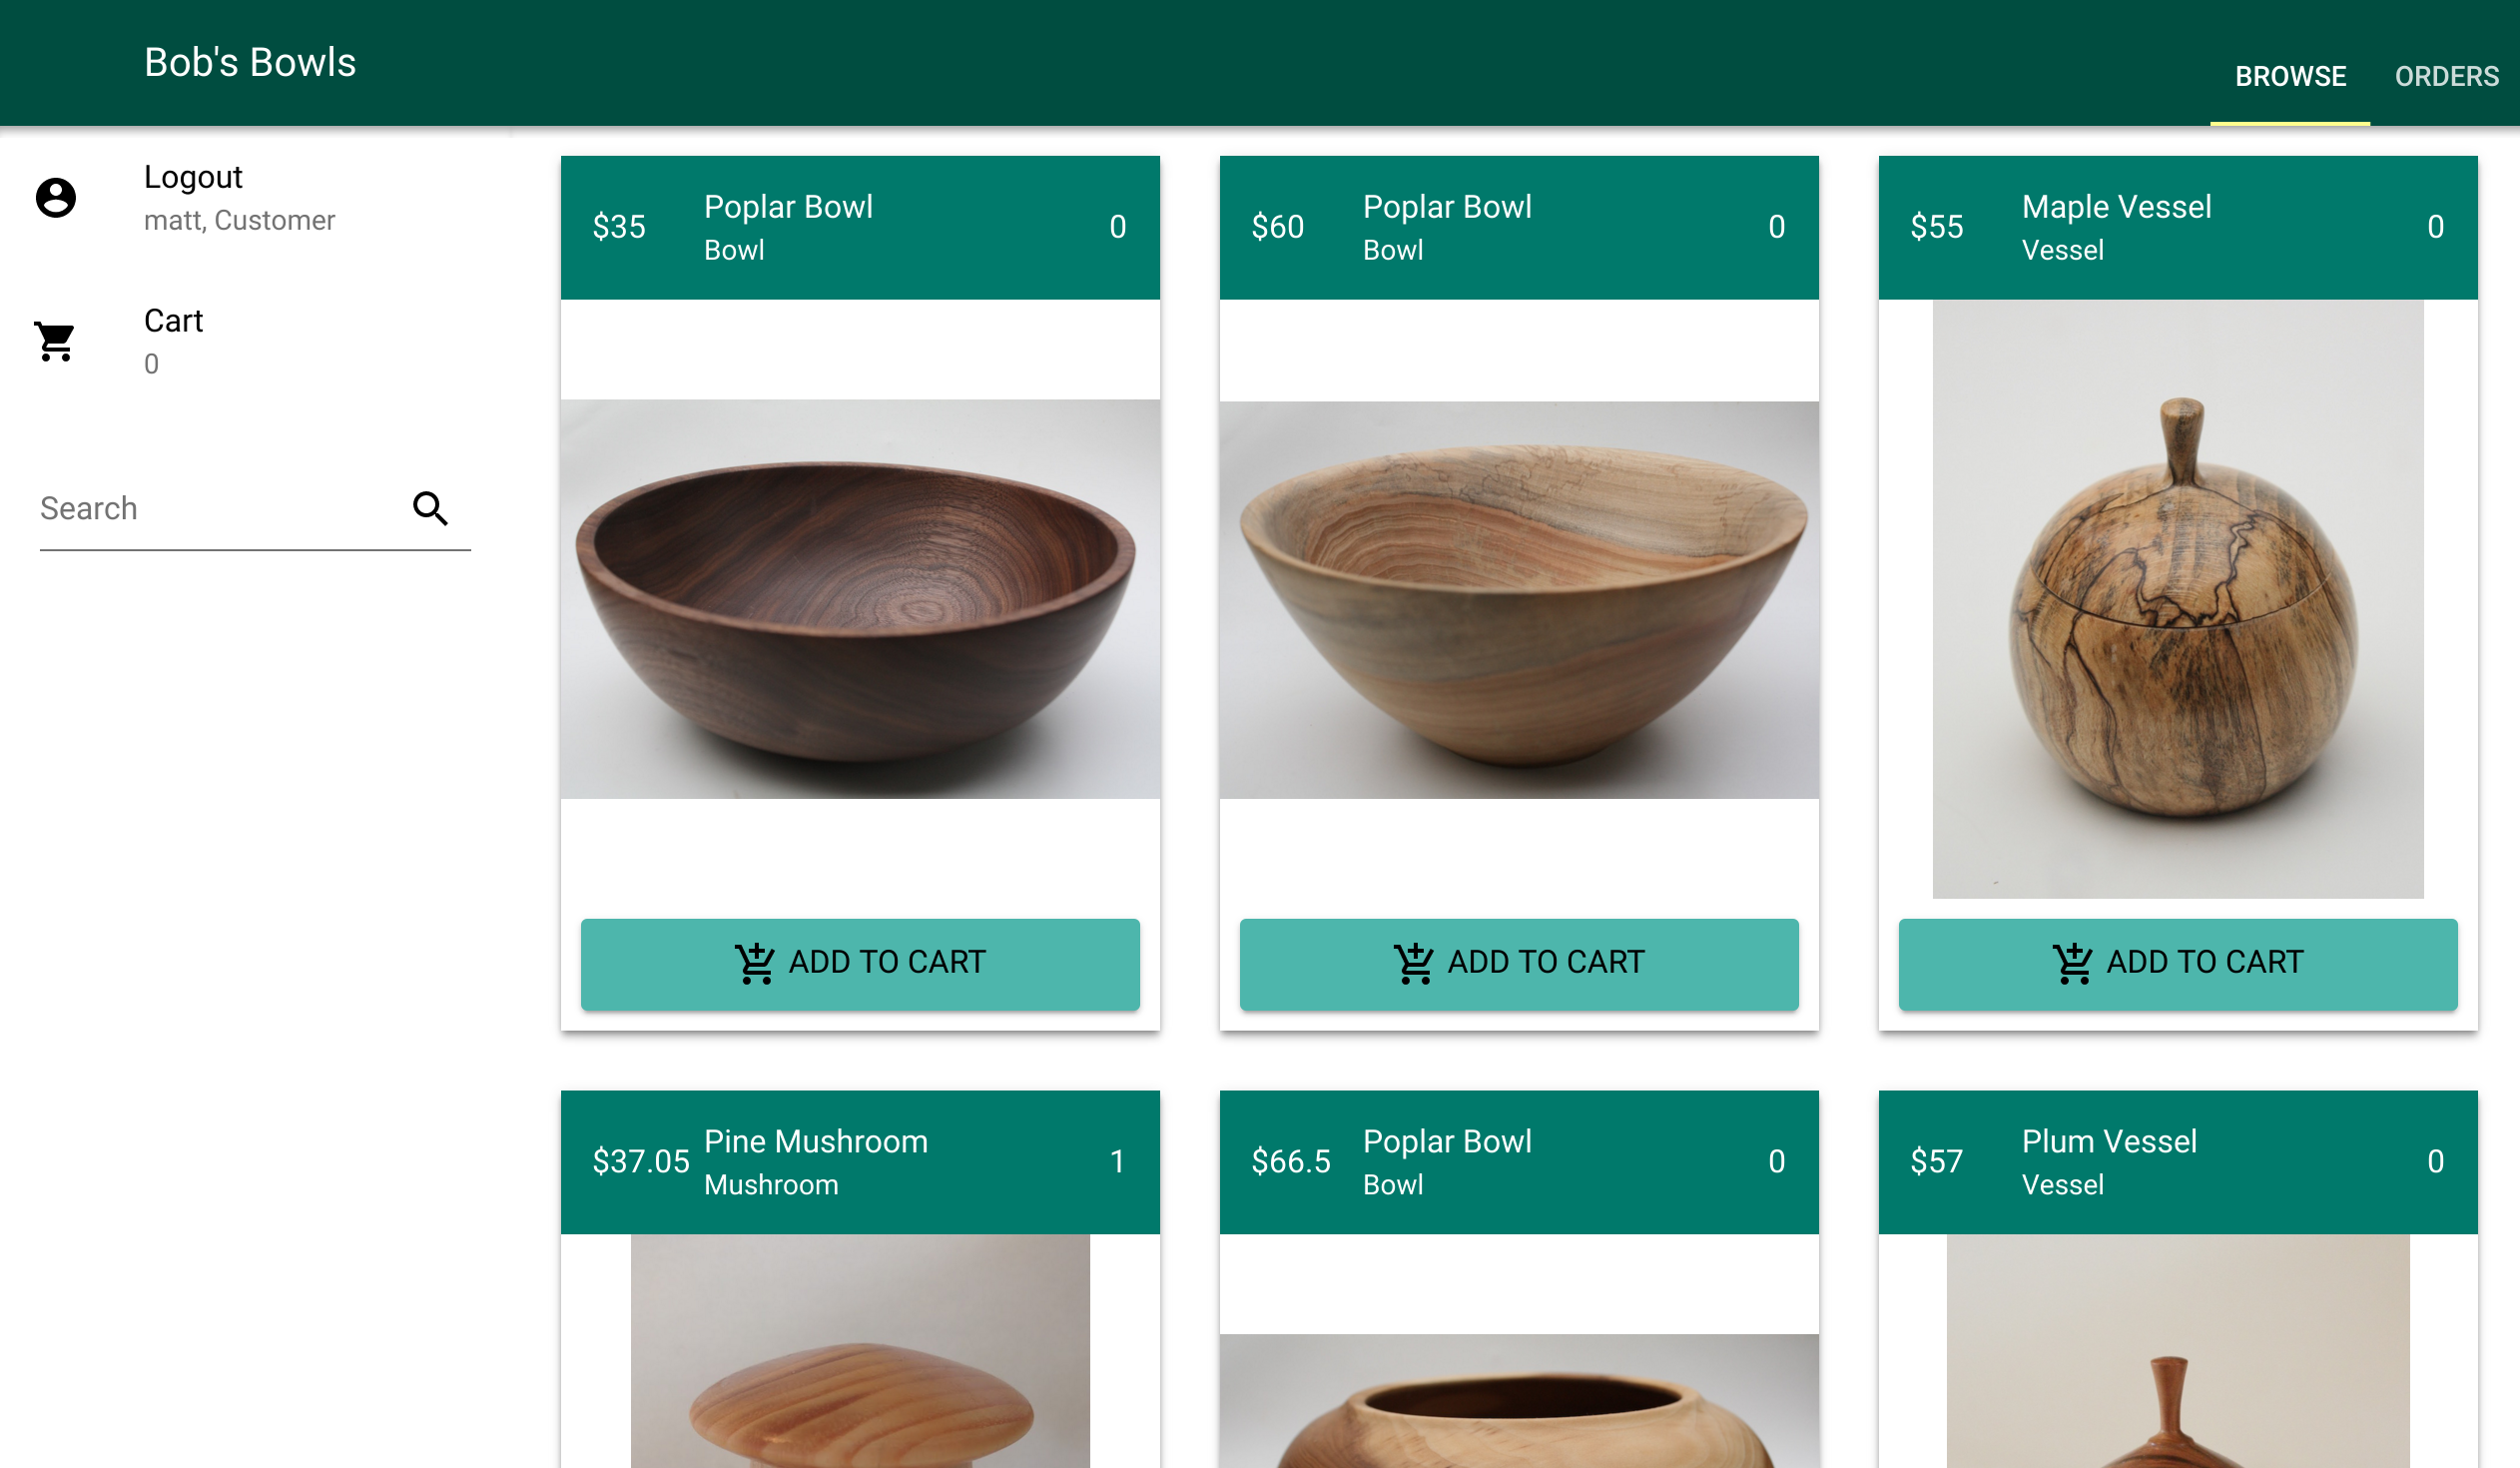
\includegraphics[width=.8\textwidth]{user-login}
\caption{What a lowest access level user sees after logging in.}
\label{cap-user-login}
\end{figure}


\subsubsection{After Manager Login}
\begin{figure}[H]
\centering
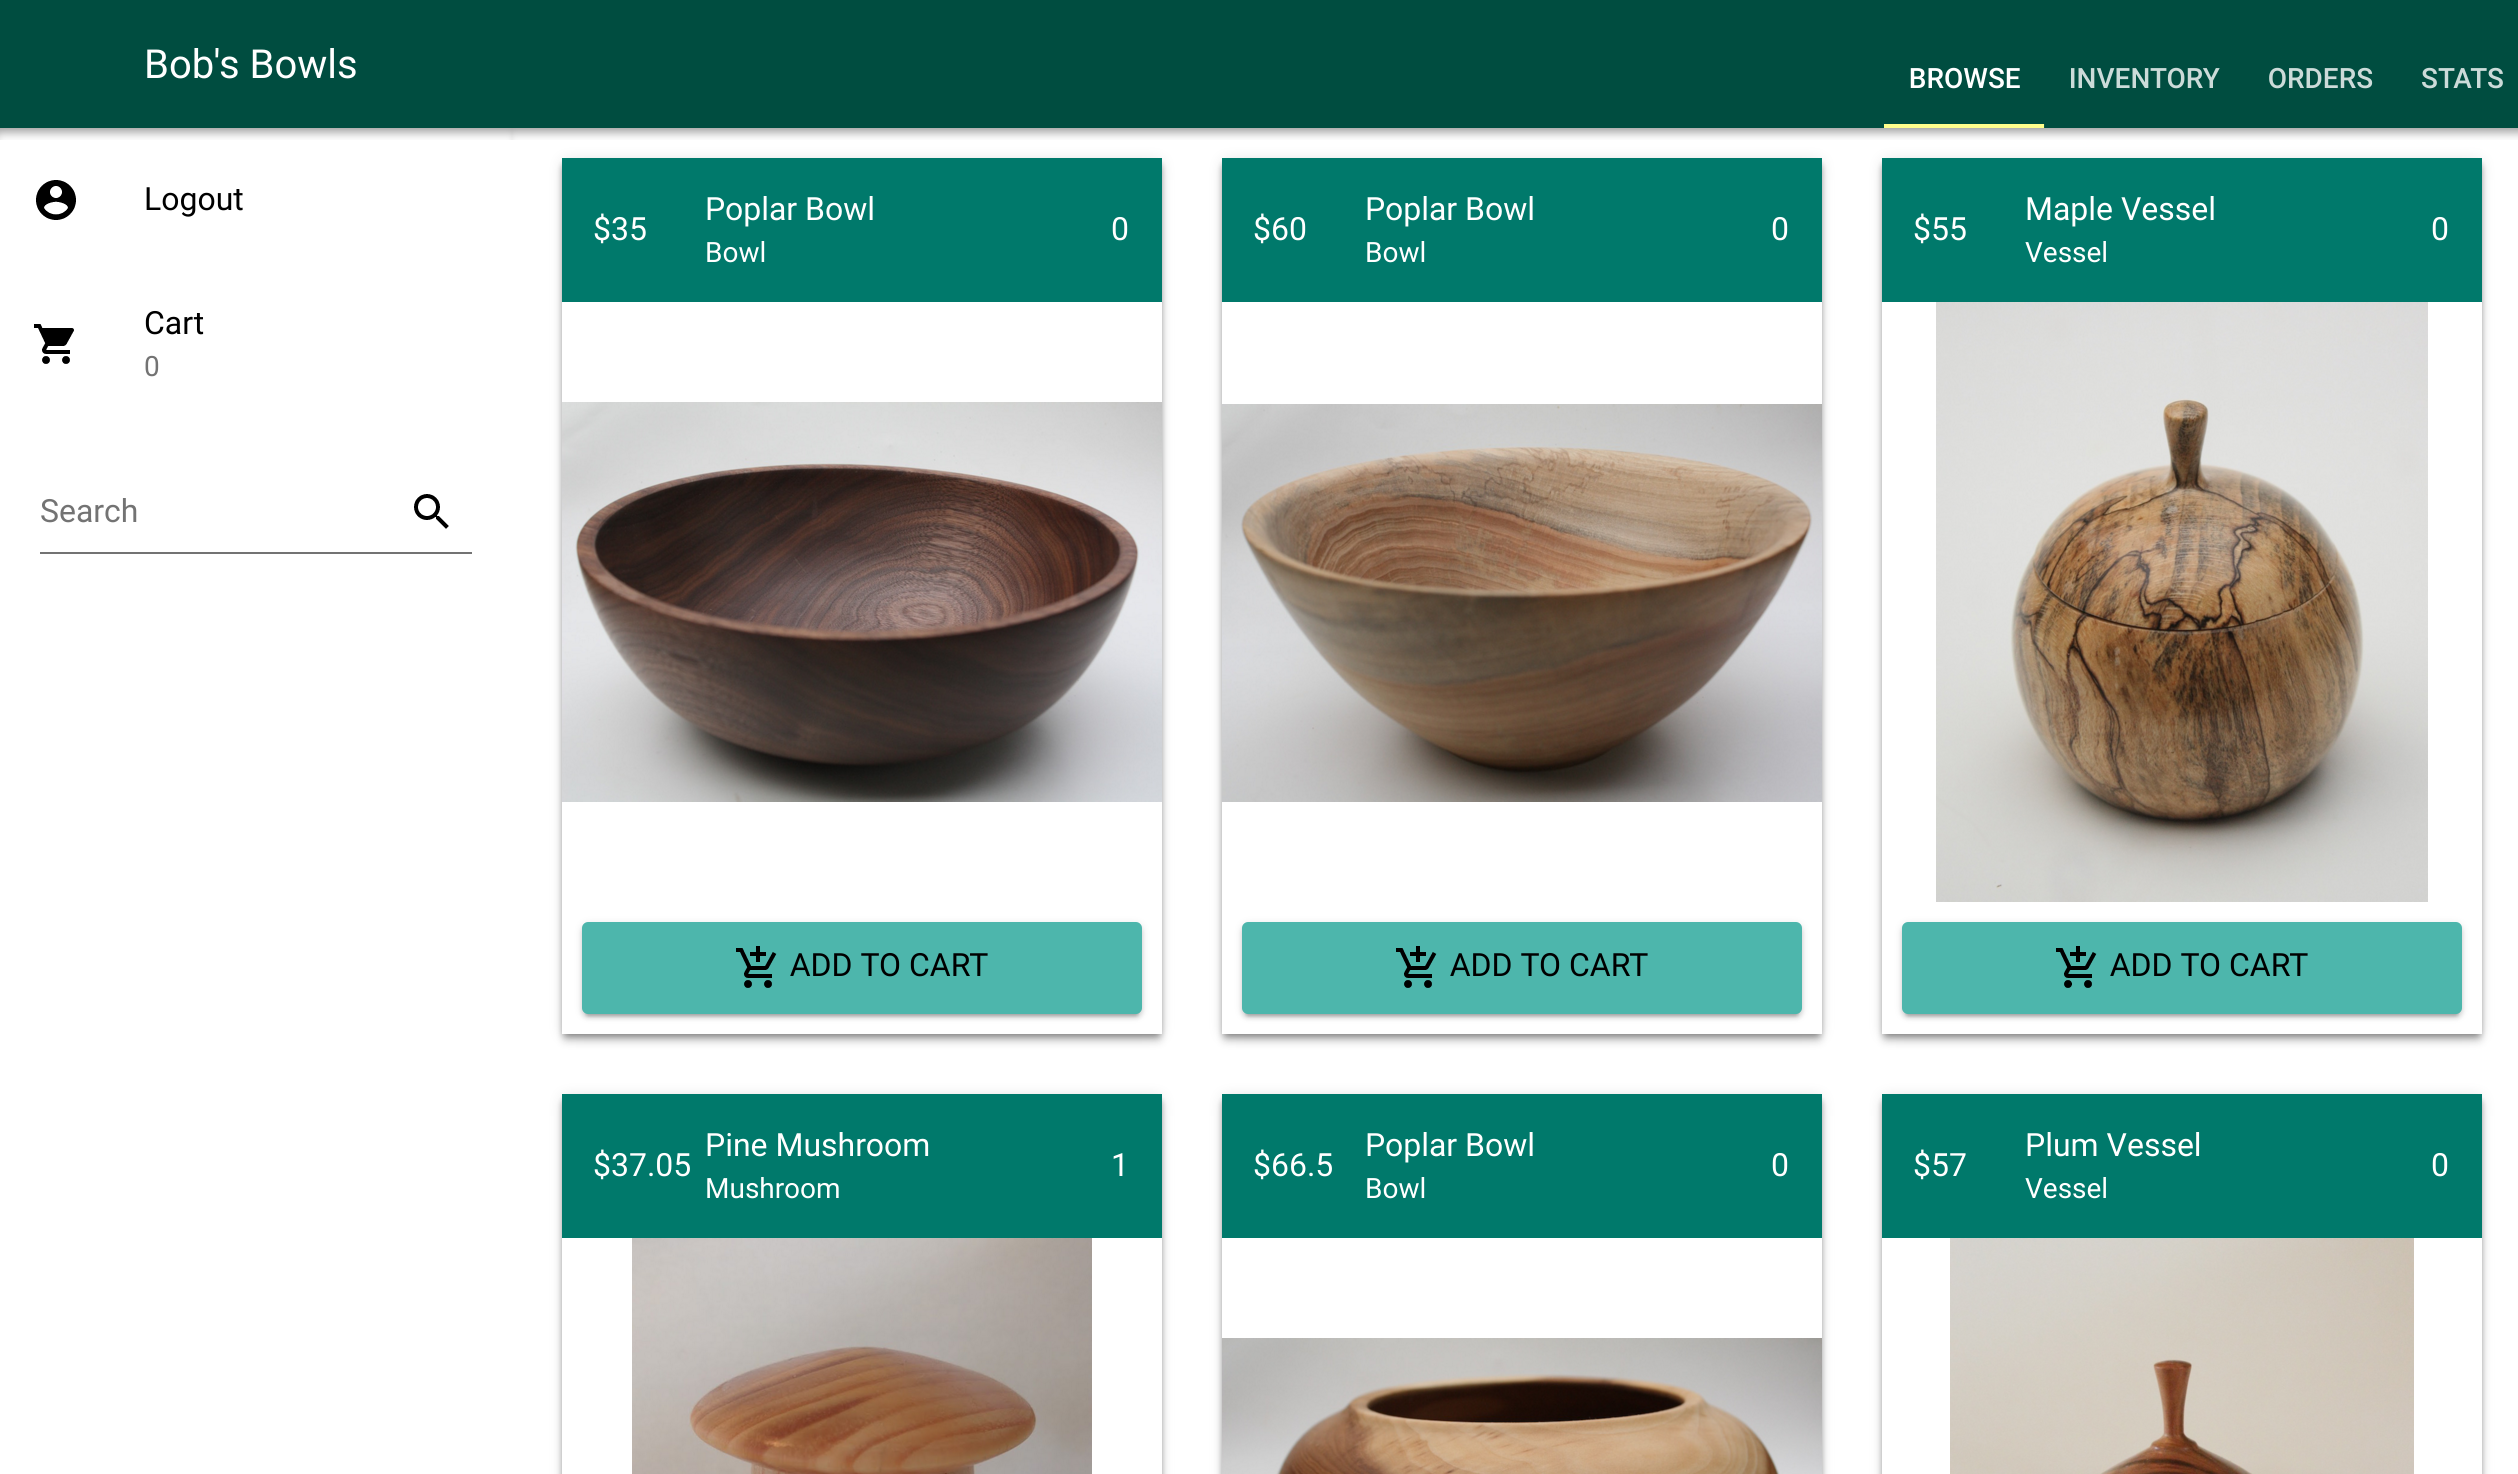
\includegraphics[width=.8\textwidth]{manager-login}
\caption{What a manager sees after logging in.}
\label{cap-manager-login}
\end{figure}


\subsubsection{Search}
\begin{figure}[H]
\centering
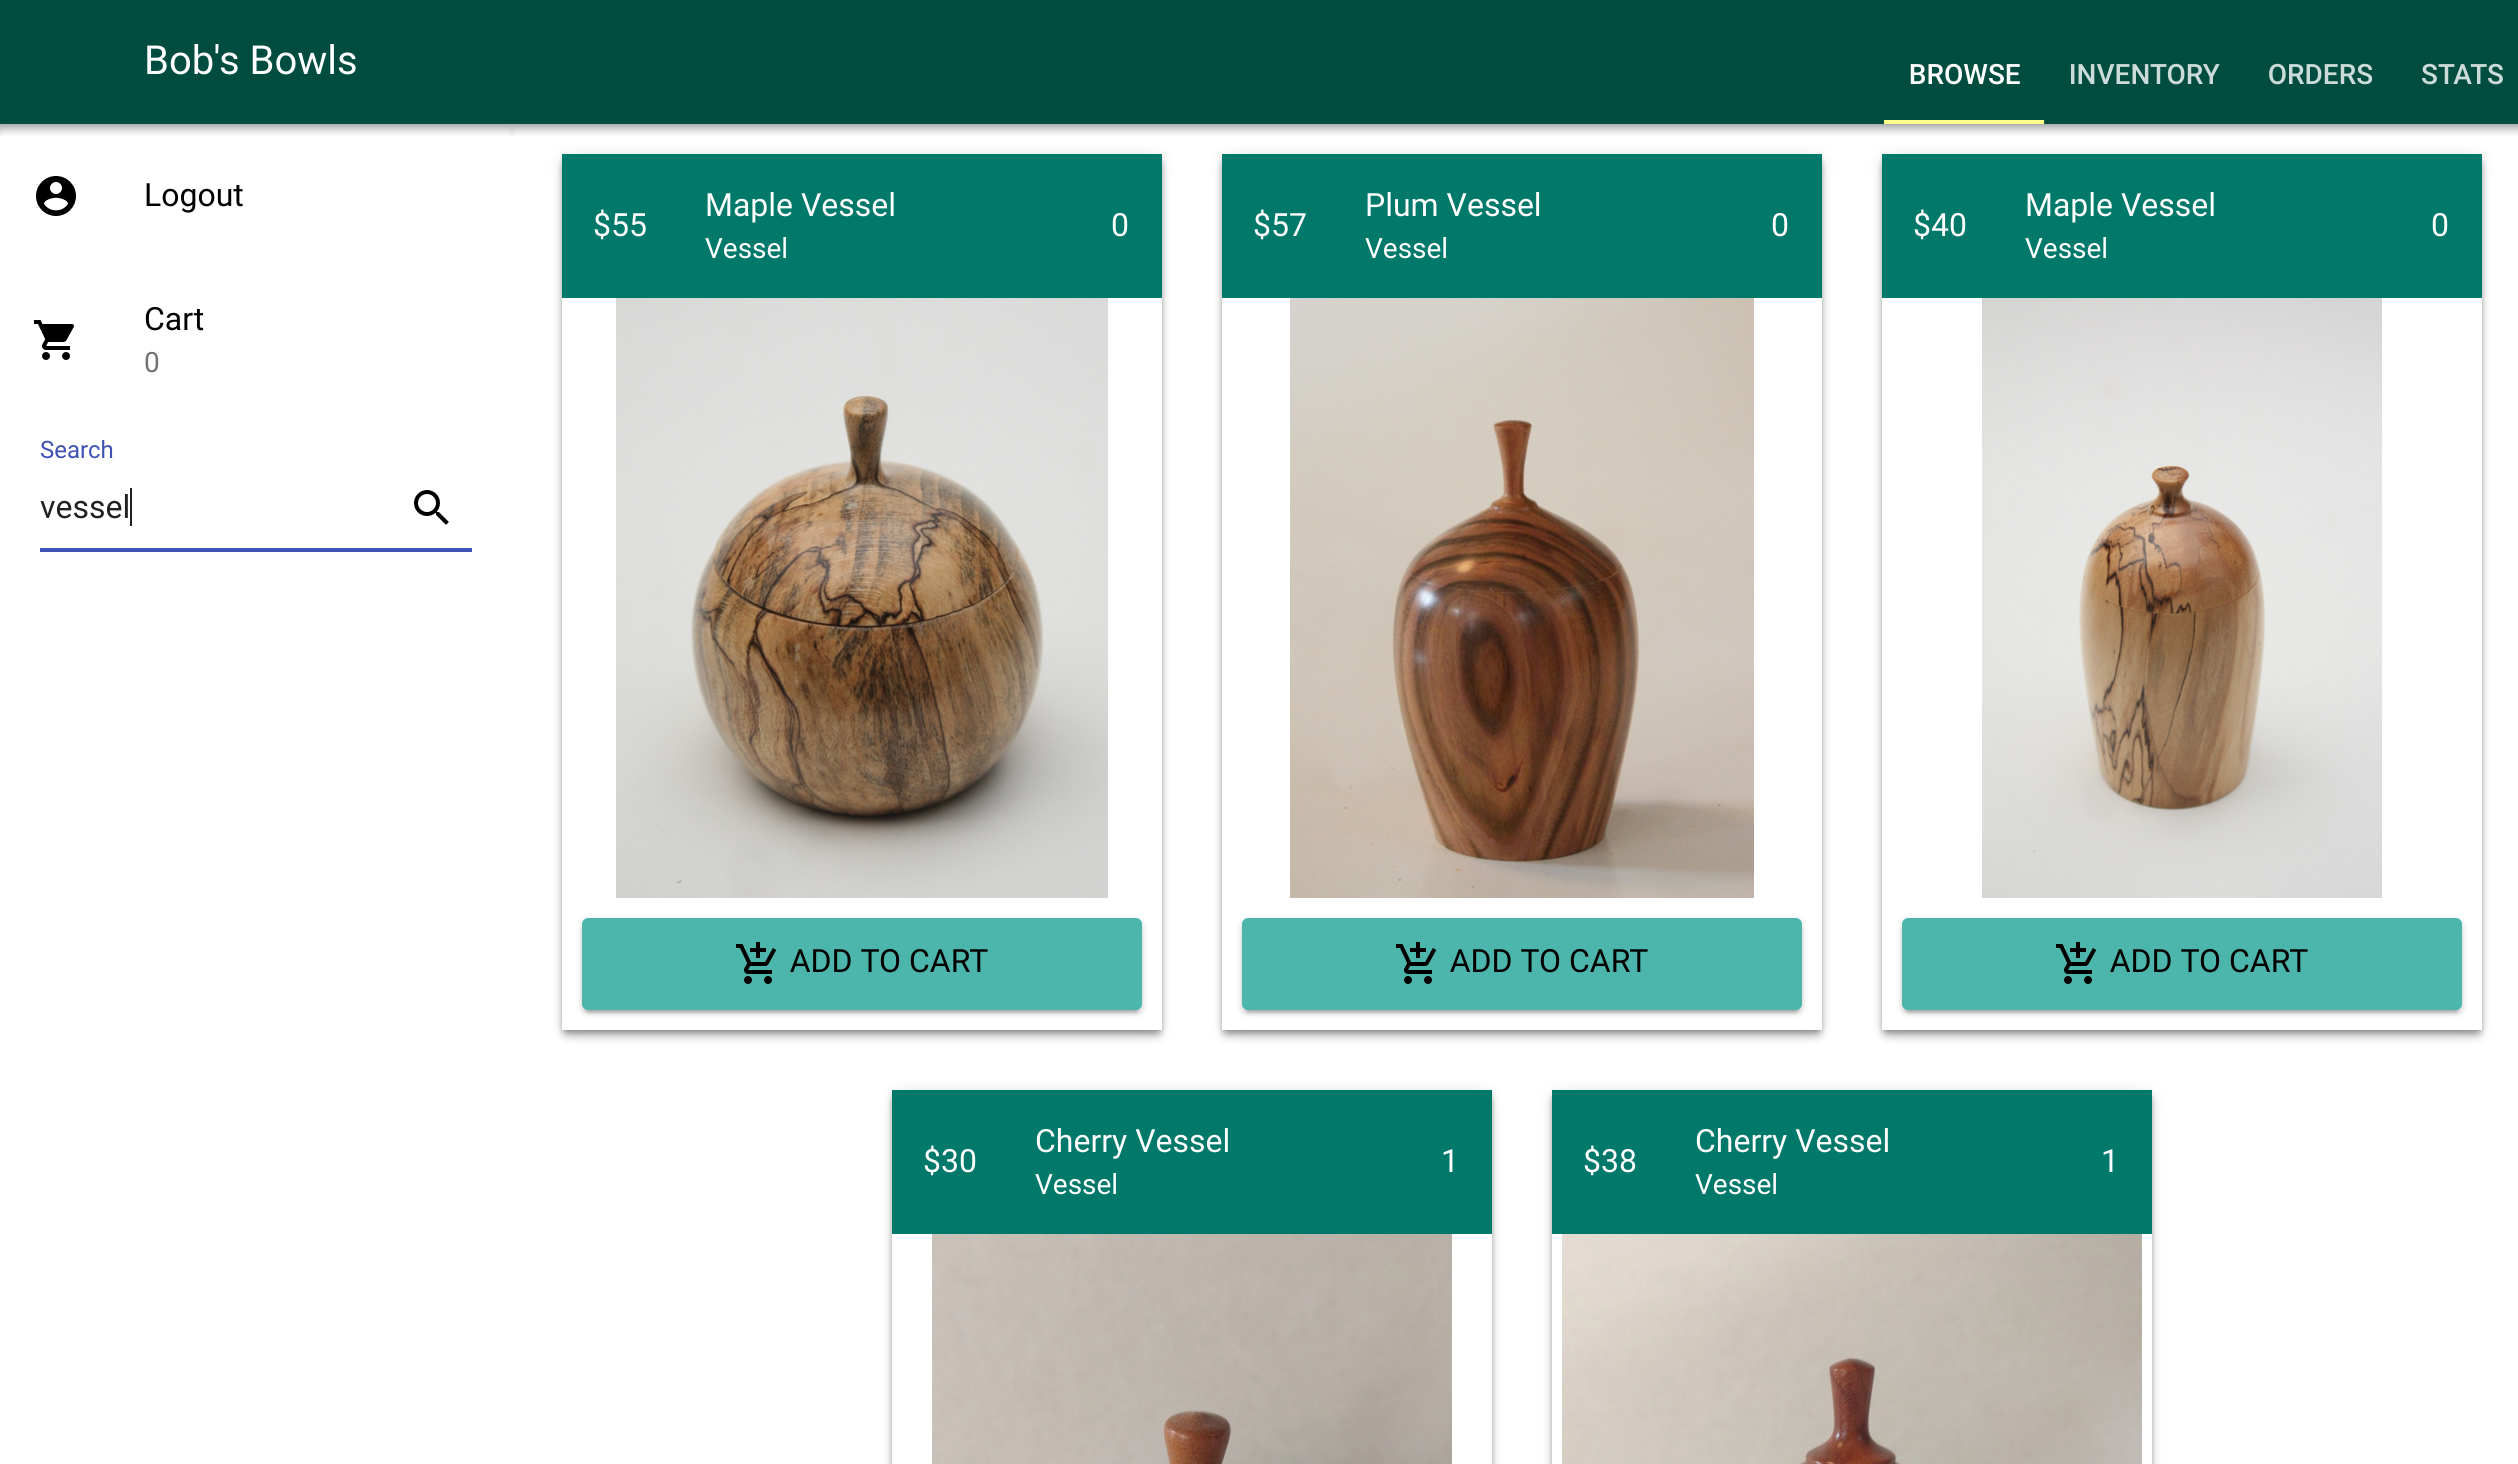
\includegraphics[width=.8\textwidth]{search}
\caption{What filtering by type looks like.}
\label{cap-search}
\end{figure}


\subsubsection{Cart}
\begin{figure}[H]
\centering
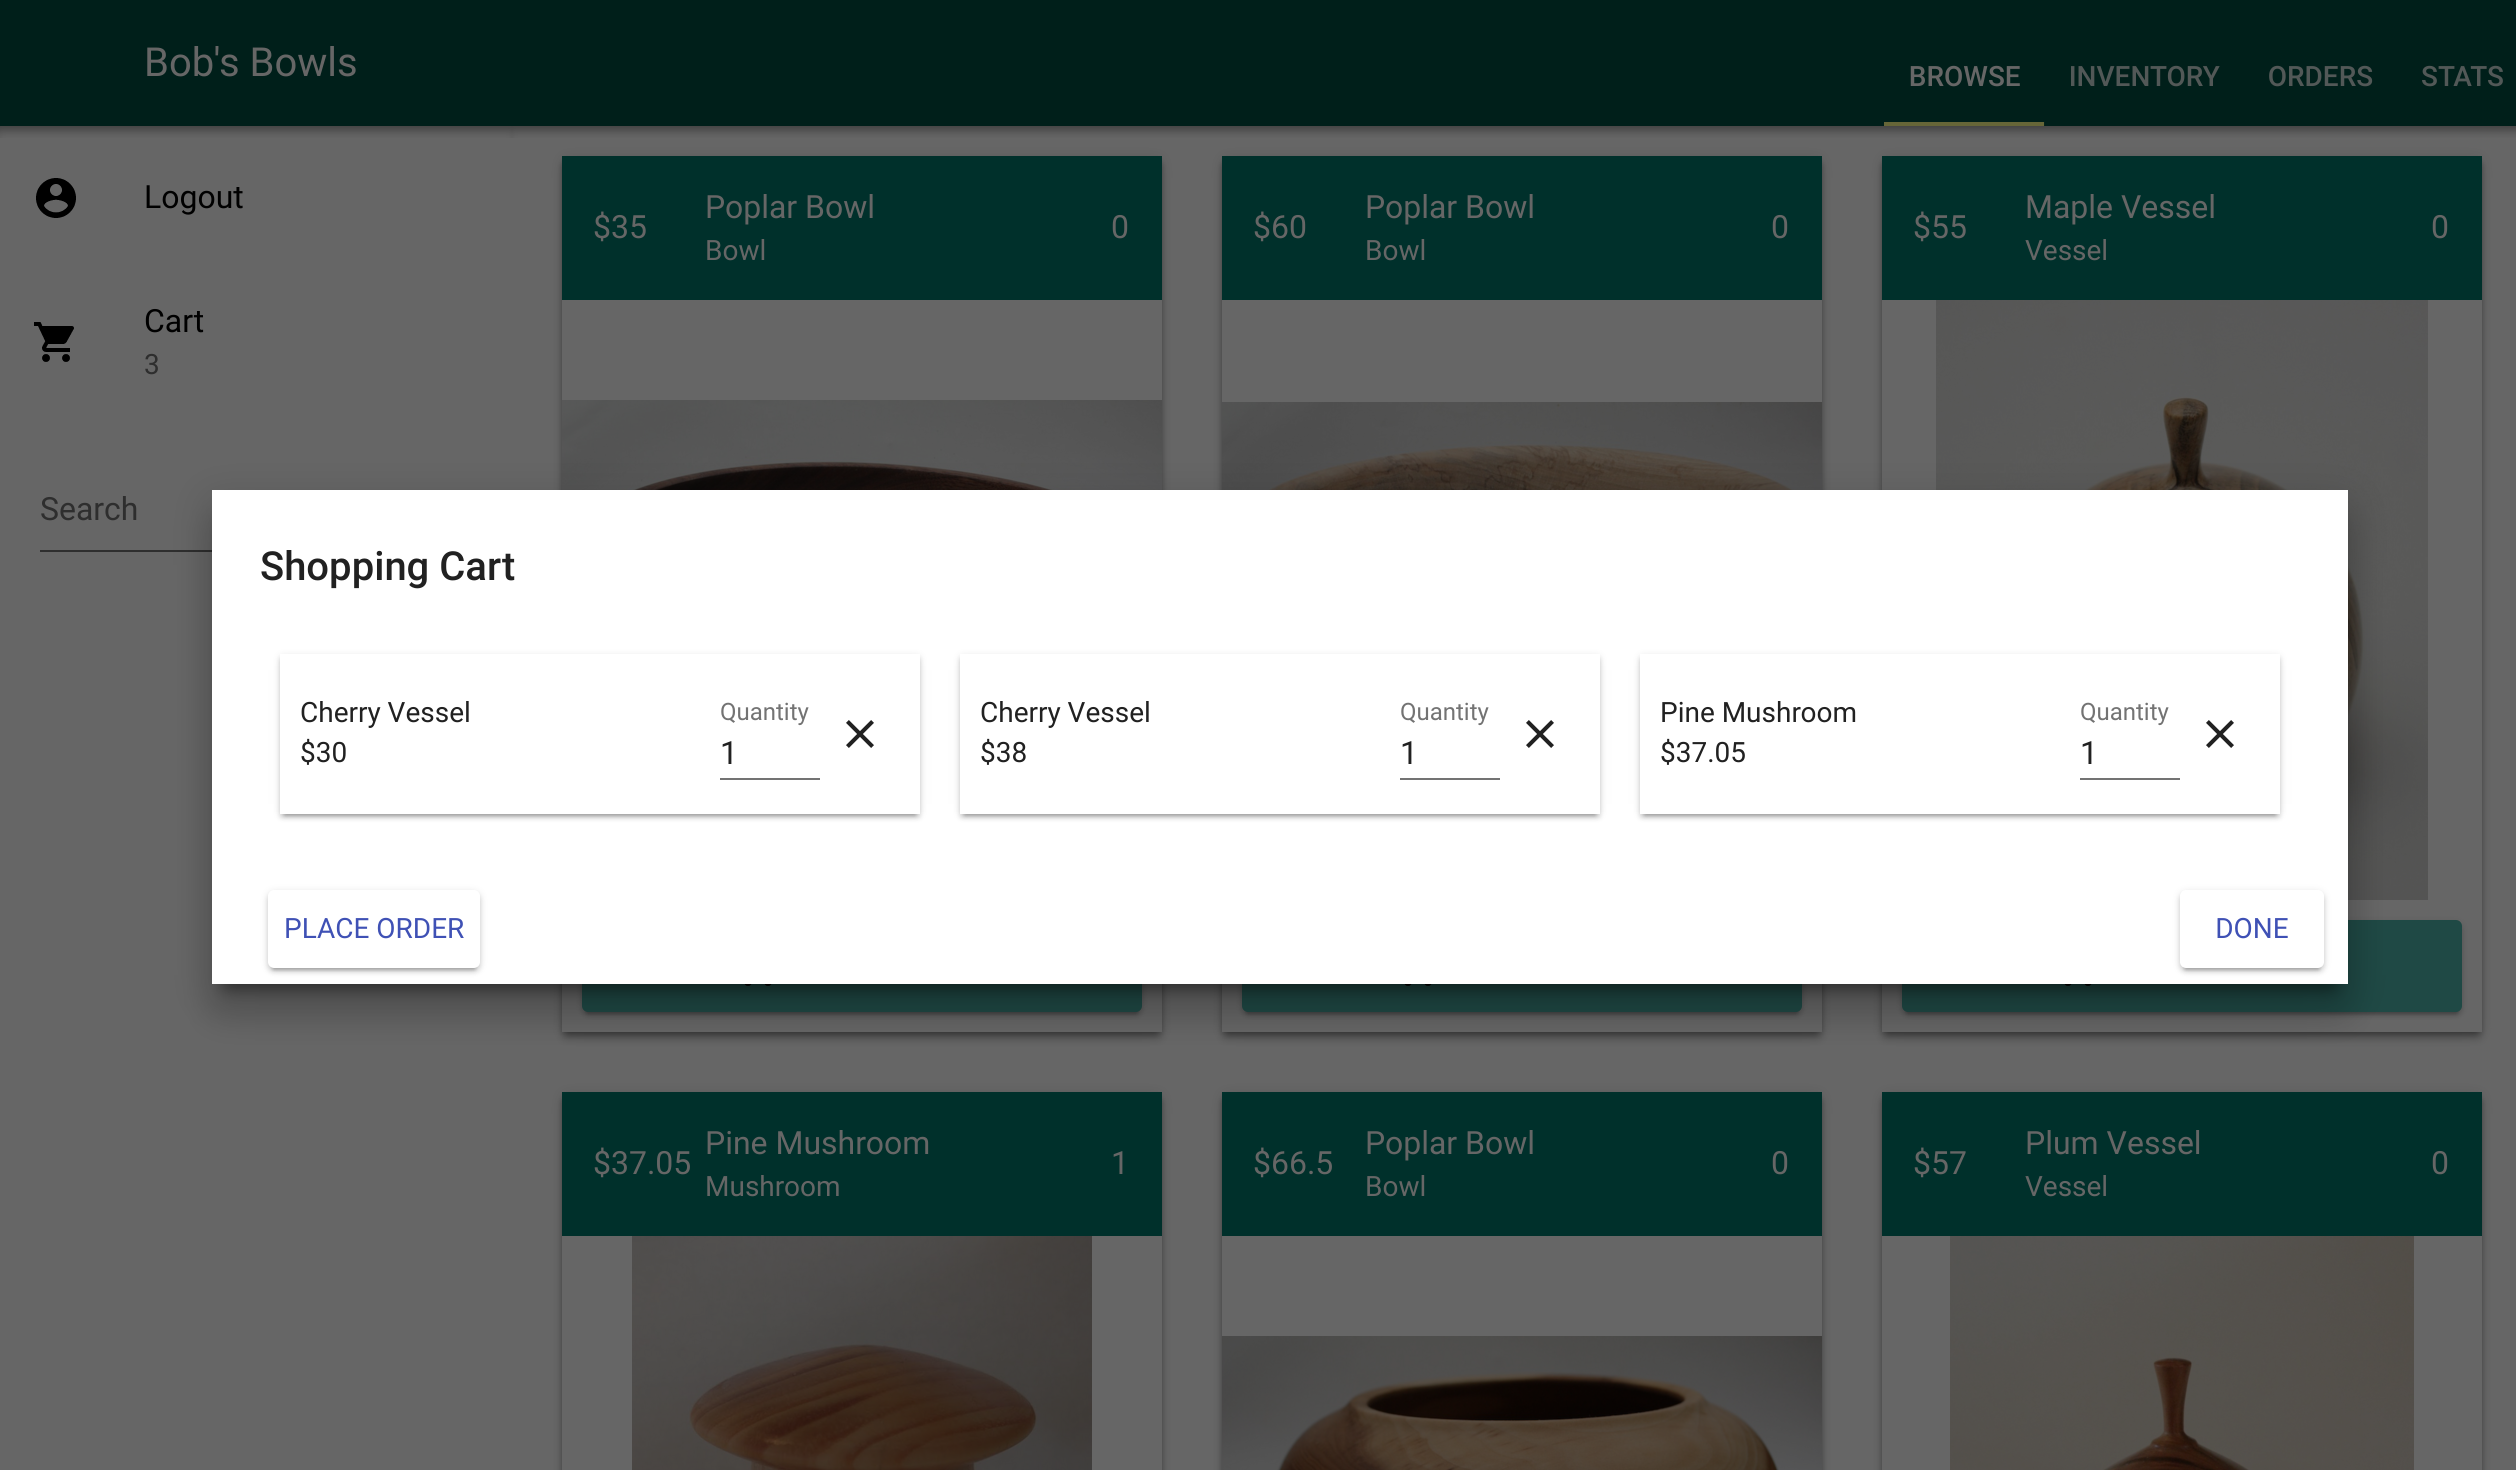
\includegraphics[width=.8\textwidth]{cart}
\caption{How items appear when in the cart.}
\label{cap-cart}
\end{figure}

\subsubsection{Users Orders Page}
\begin{figure}[H]
\centering
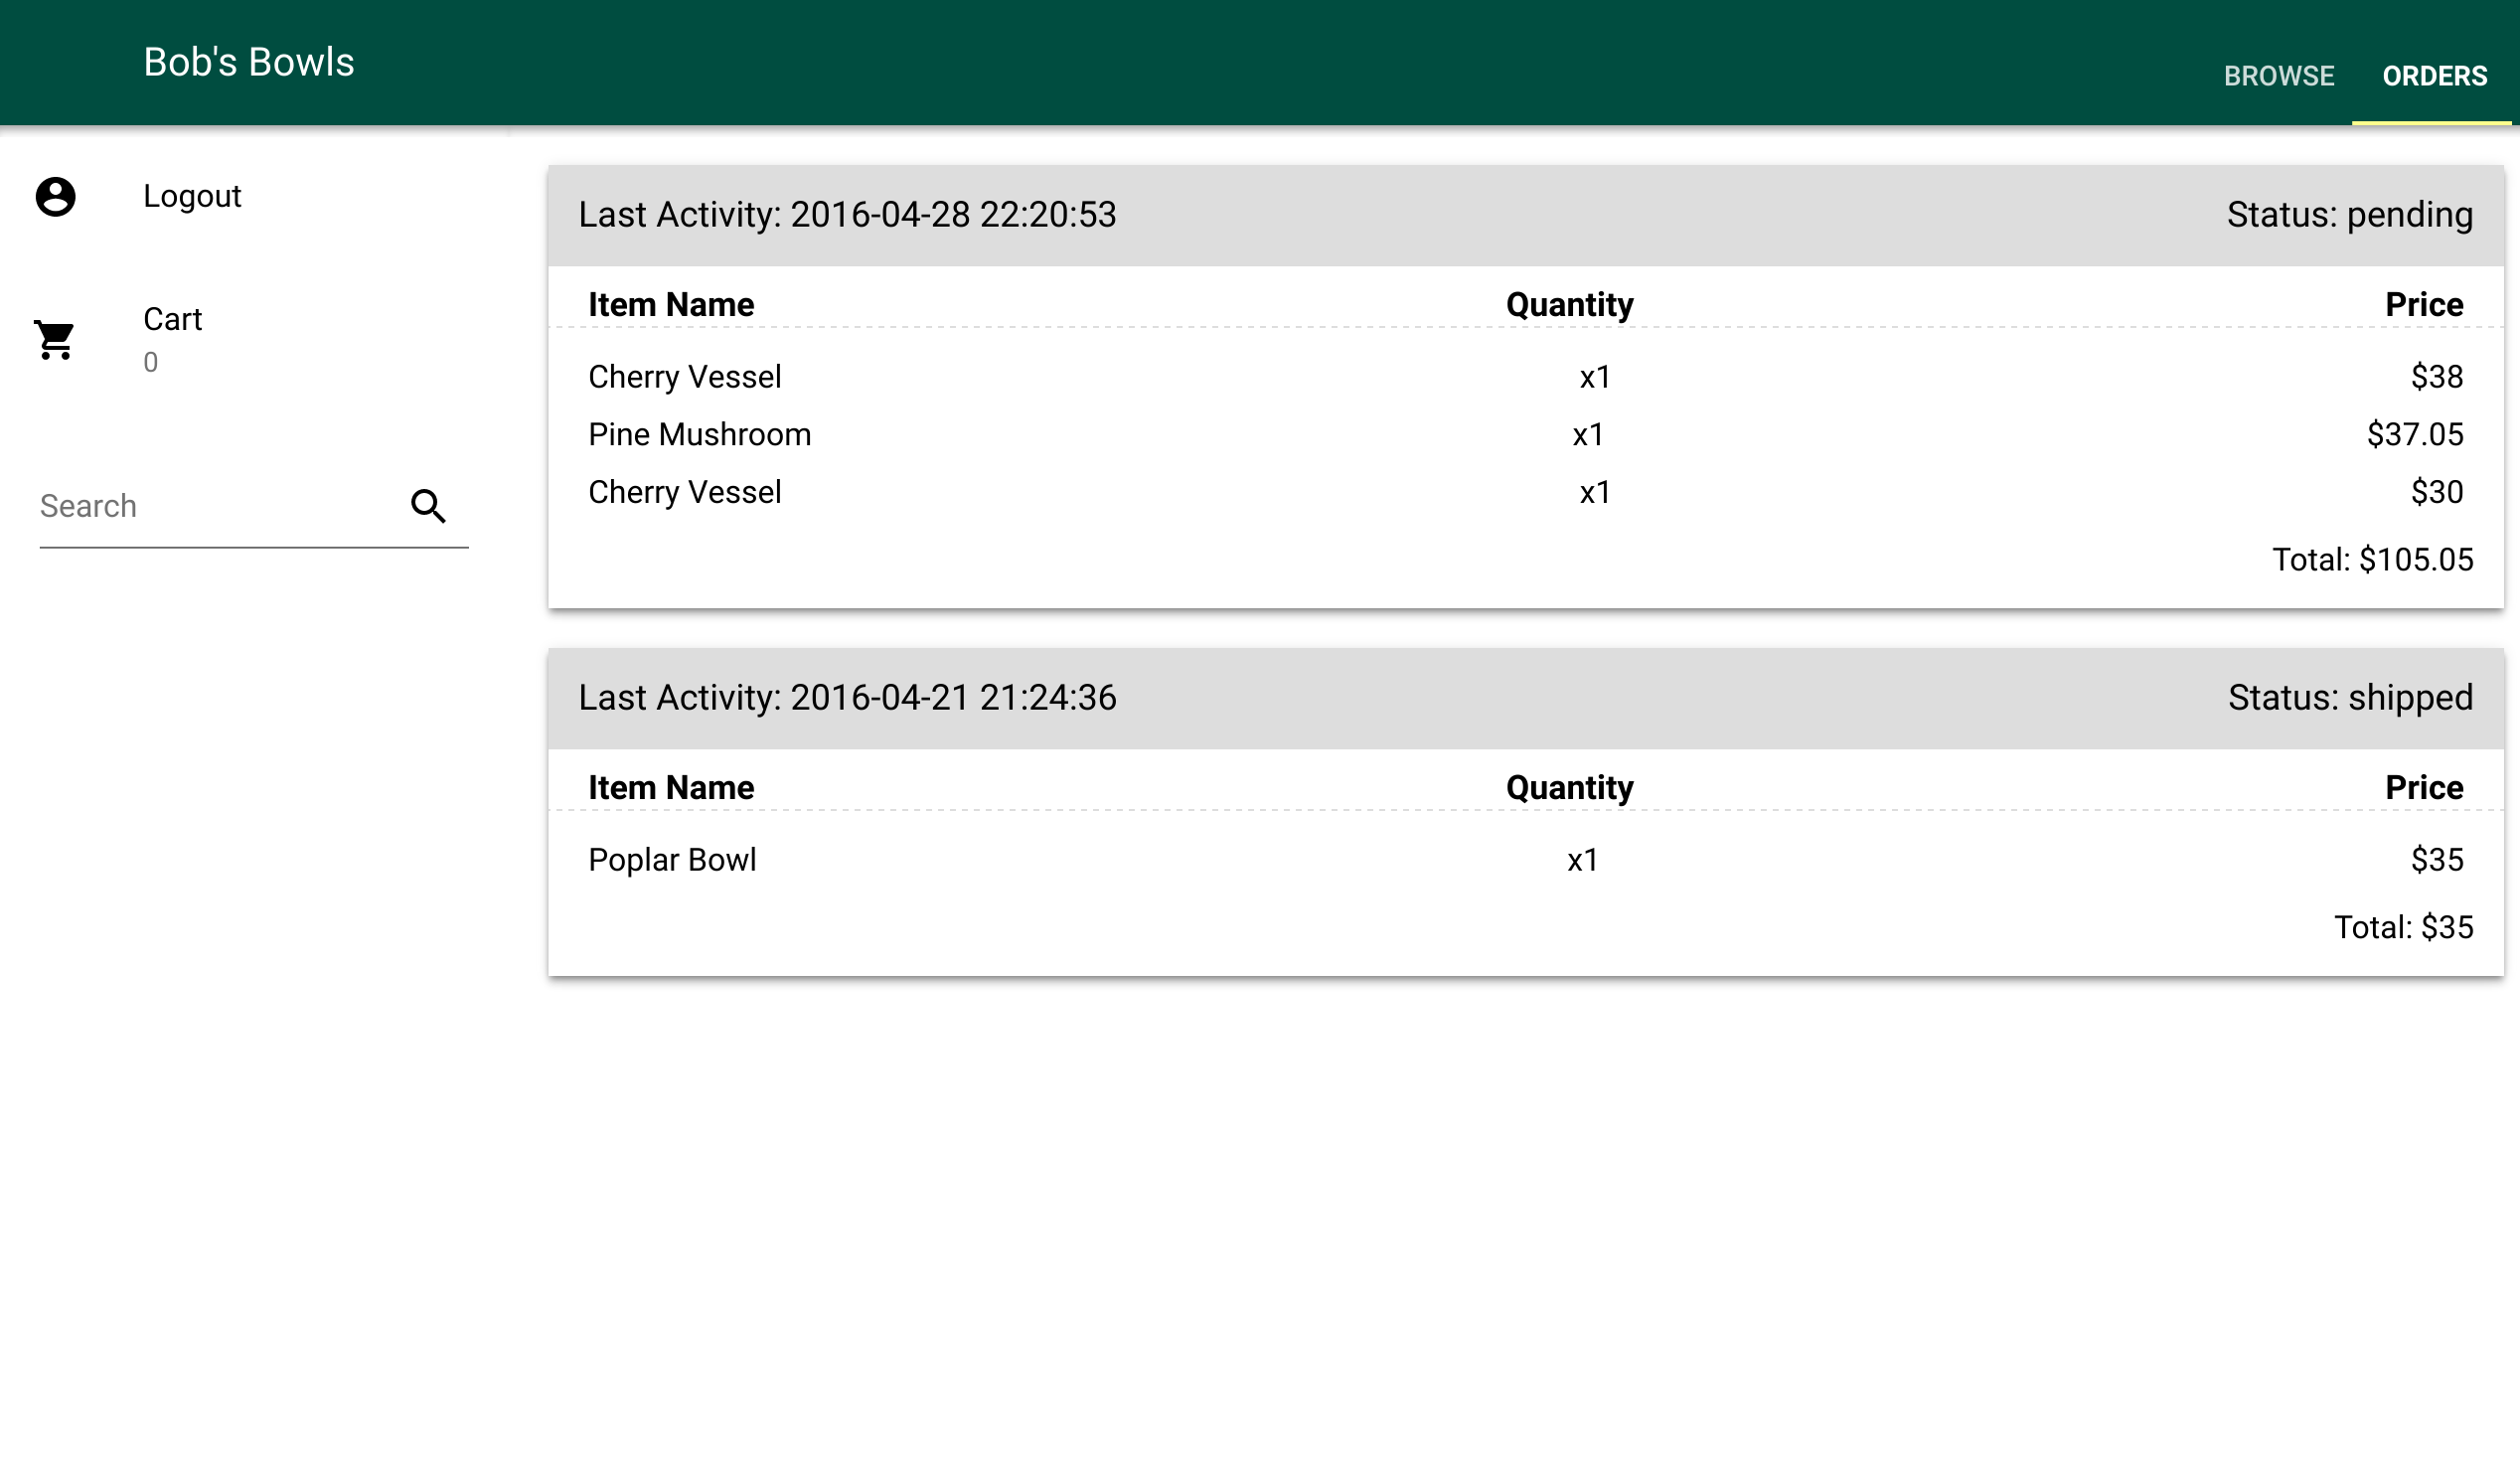
\includegraphics[width=.8\textwidth]{user-orders}
\caption{Viewing past orders as an ordinary user.}
\label{cap-user-orders}
\end{figure}

\subsubsection{Staff Orders Page}
\begin{figure}[H]
\centering
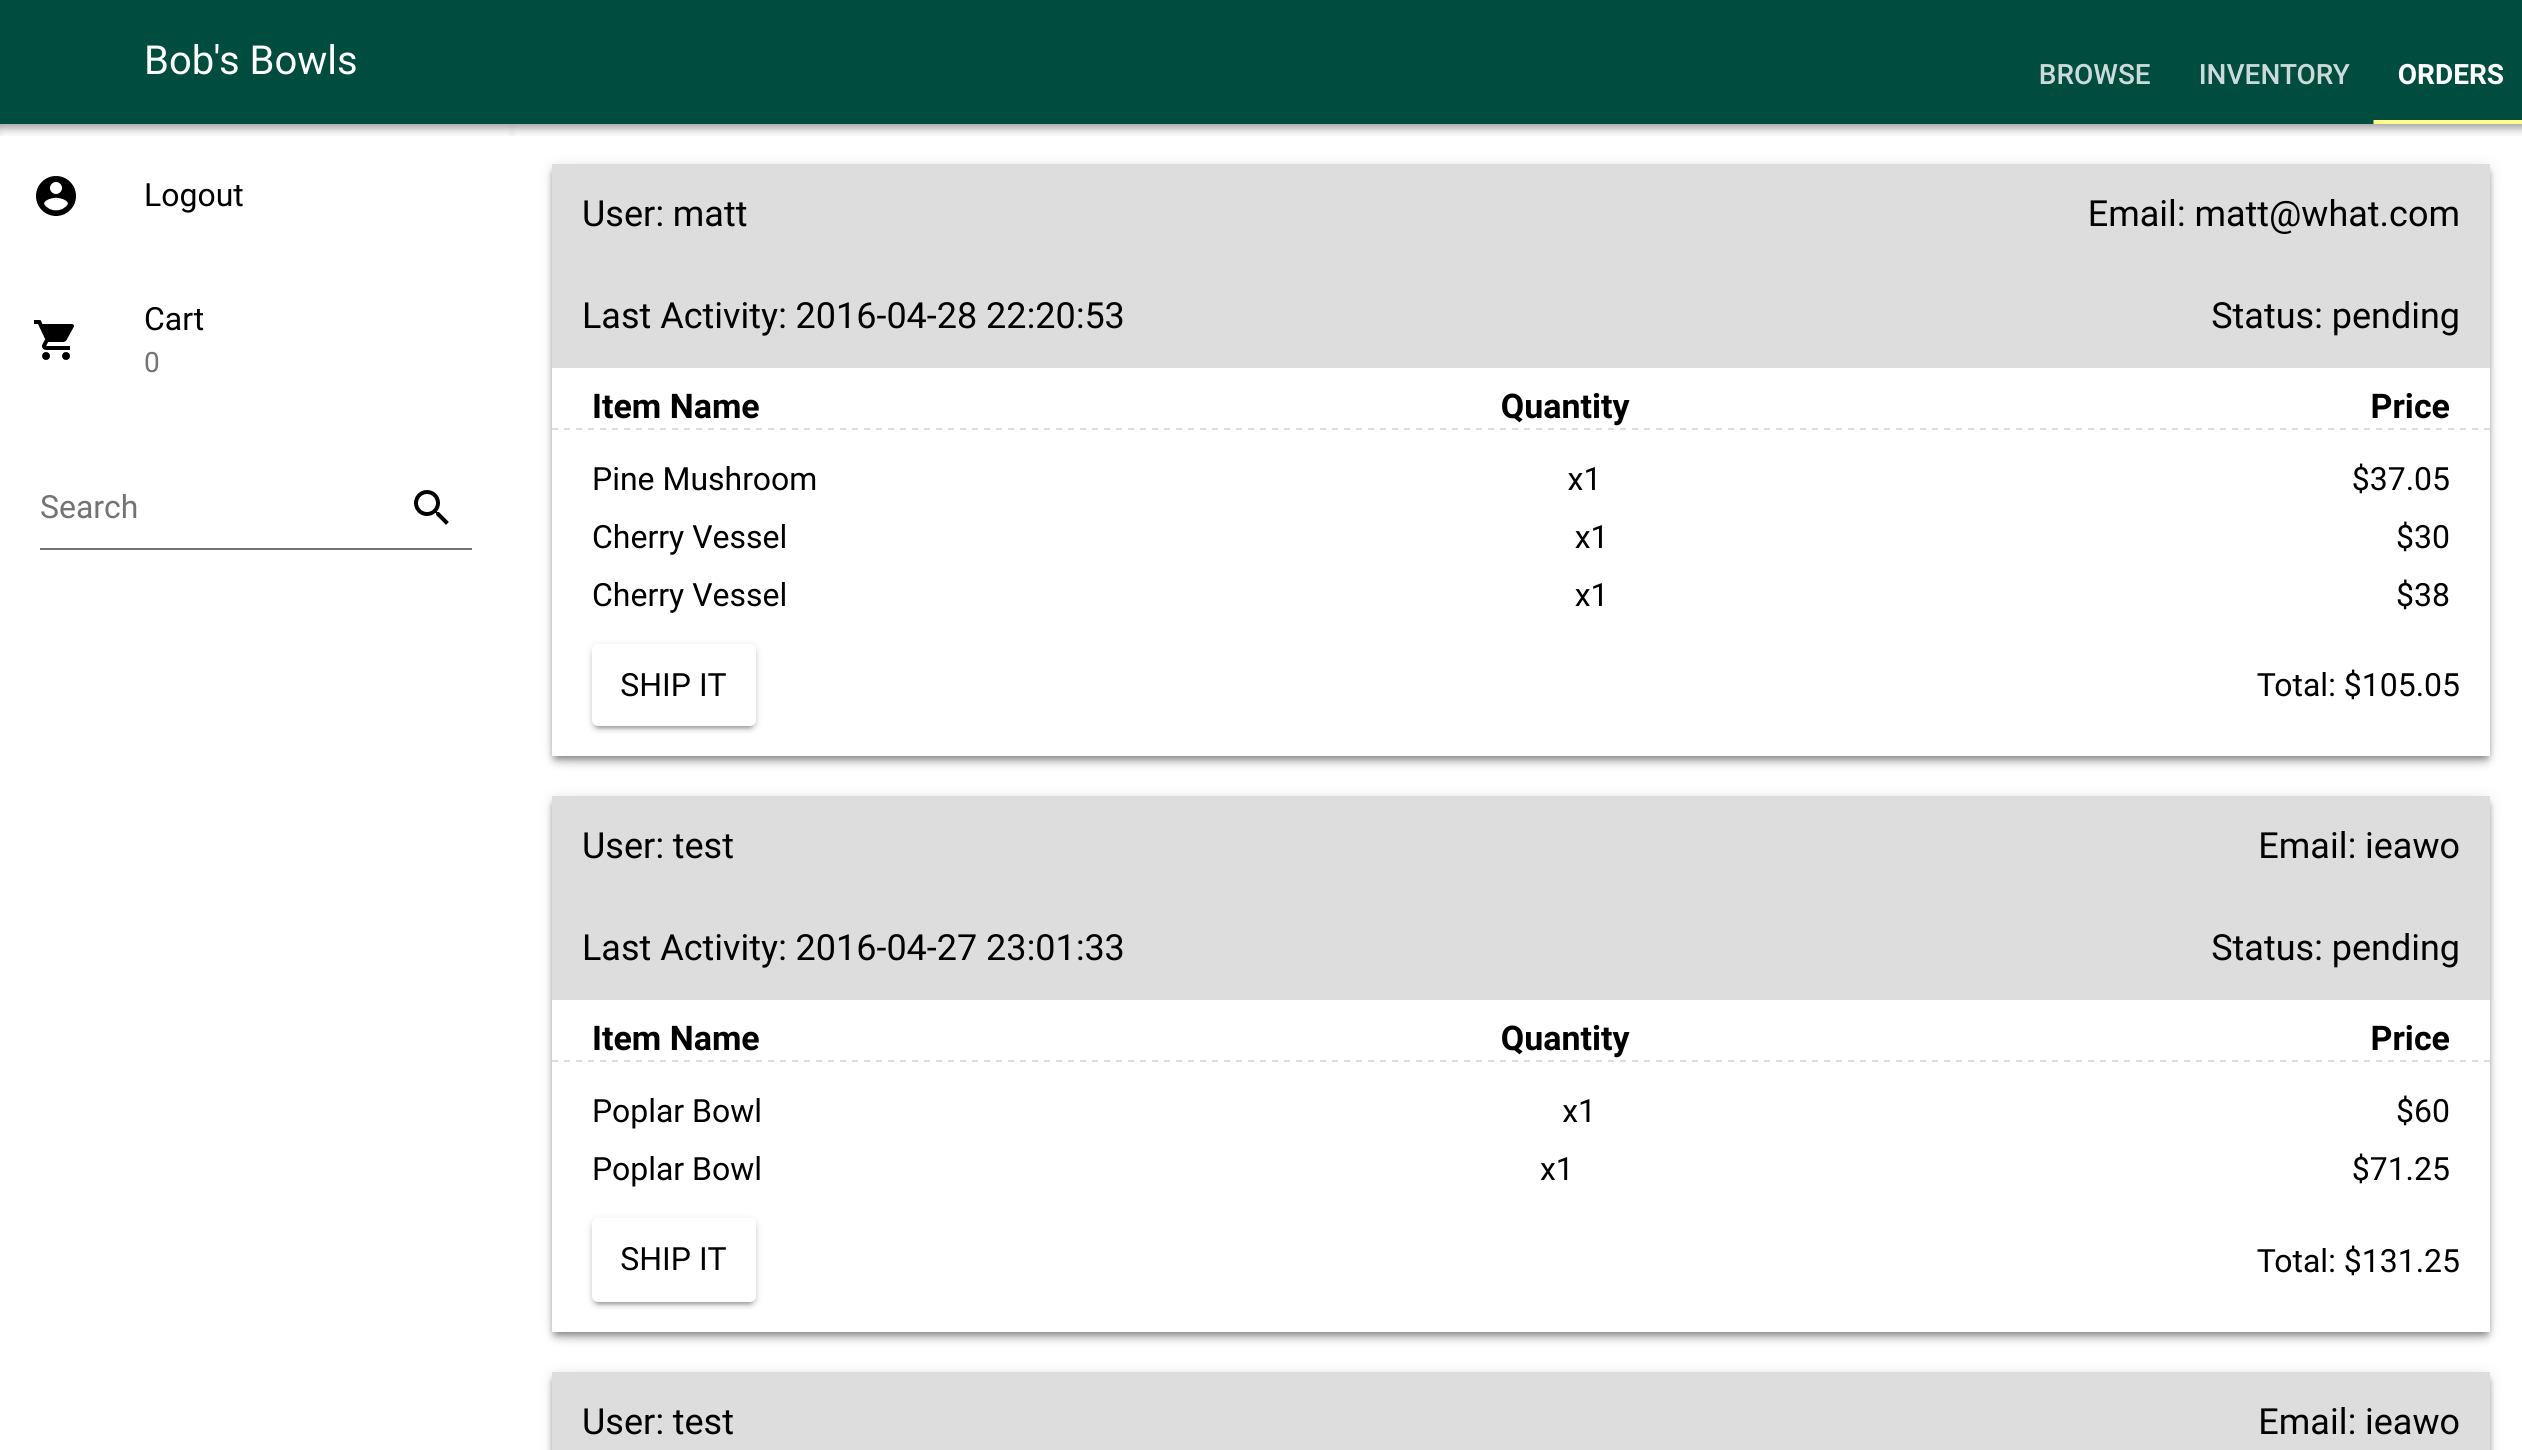
\includegraphics[width=.8\textwidth]{staff-orders}
\caption{Viewing orders as a staff member. Note the 'SHIP IT' button.}
\label{cap-staff-orders}
\end{figure}


\subsubsection{Update Inventory}
\begin{figure}[H]
\centering
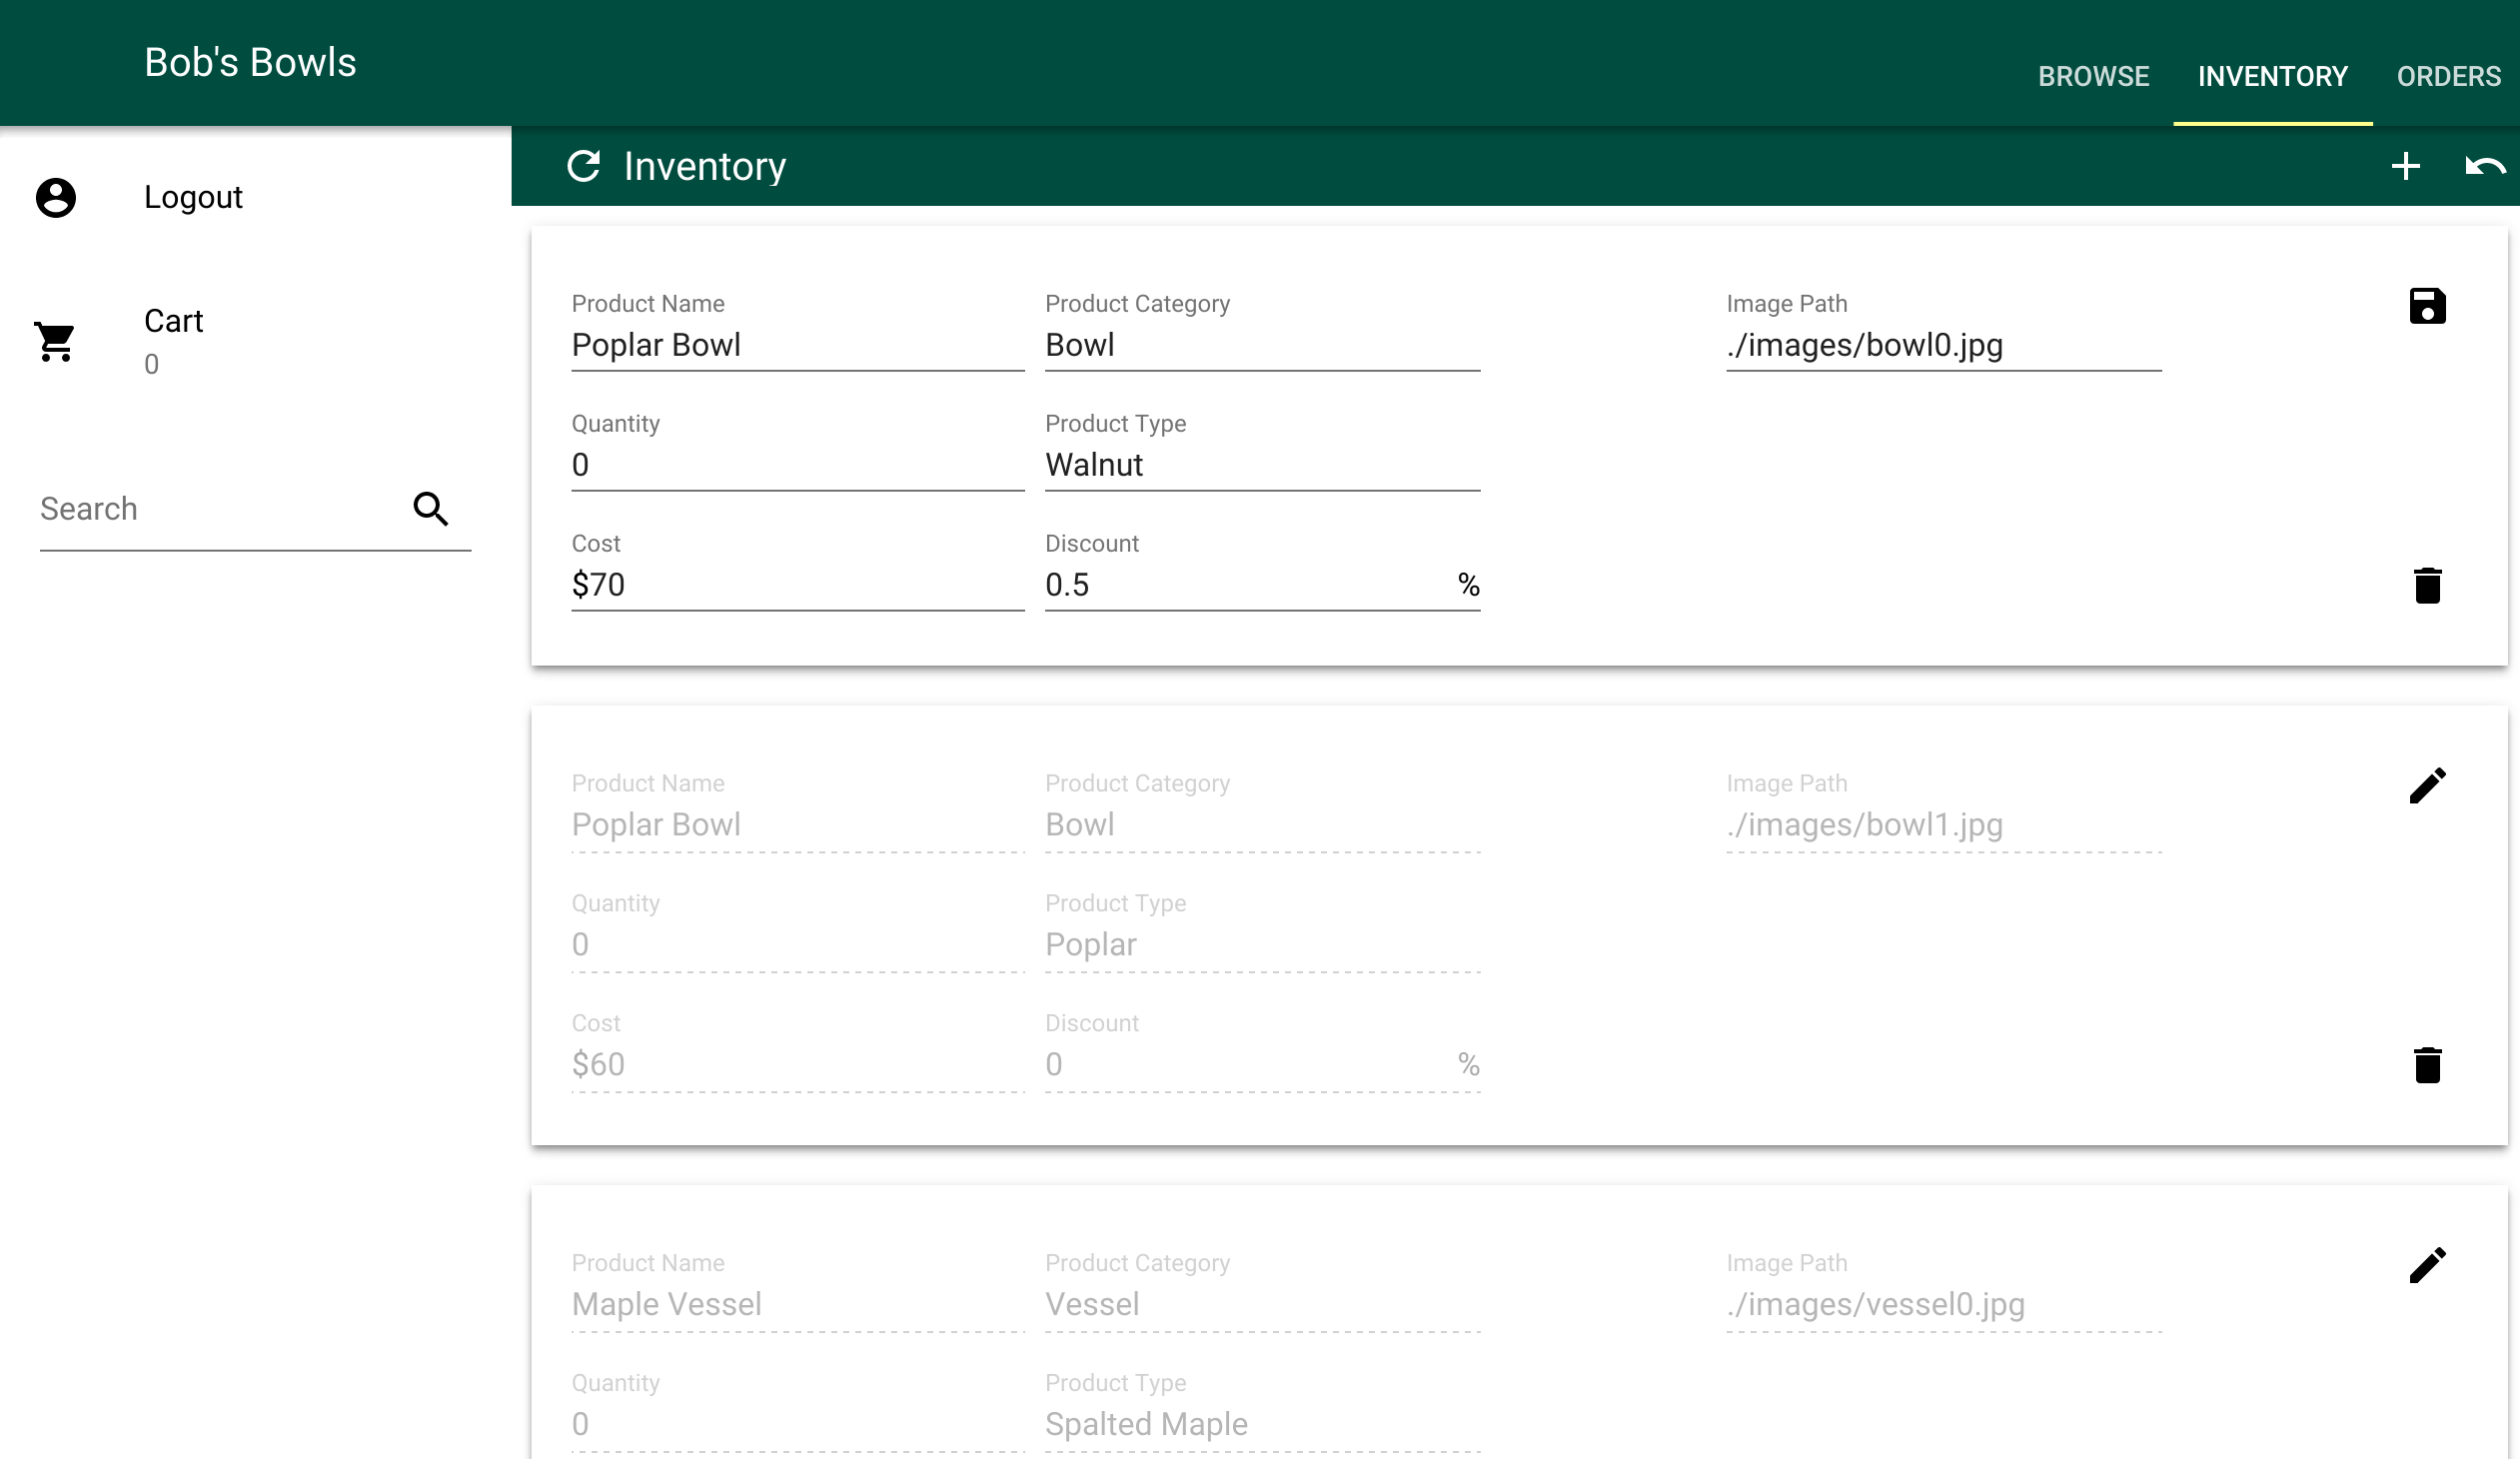
\includegraphics[width=.8\textwidth]{update-inventory}
\caption{Editing an inventory item. The item being edited is darkened.}
\label{cap-update-inventory}
\end{figure}


\subsubsection{Statistics Page}
\begin{figure}[H]
\centering
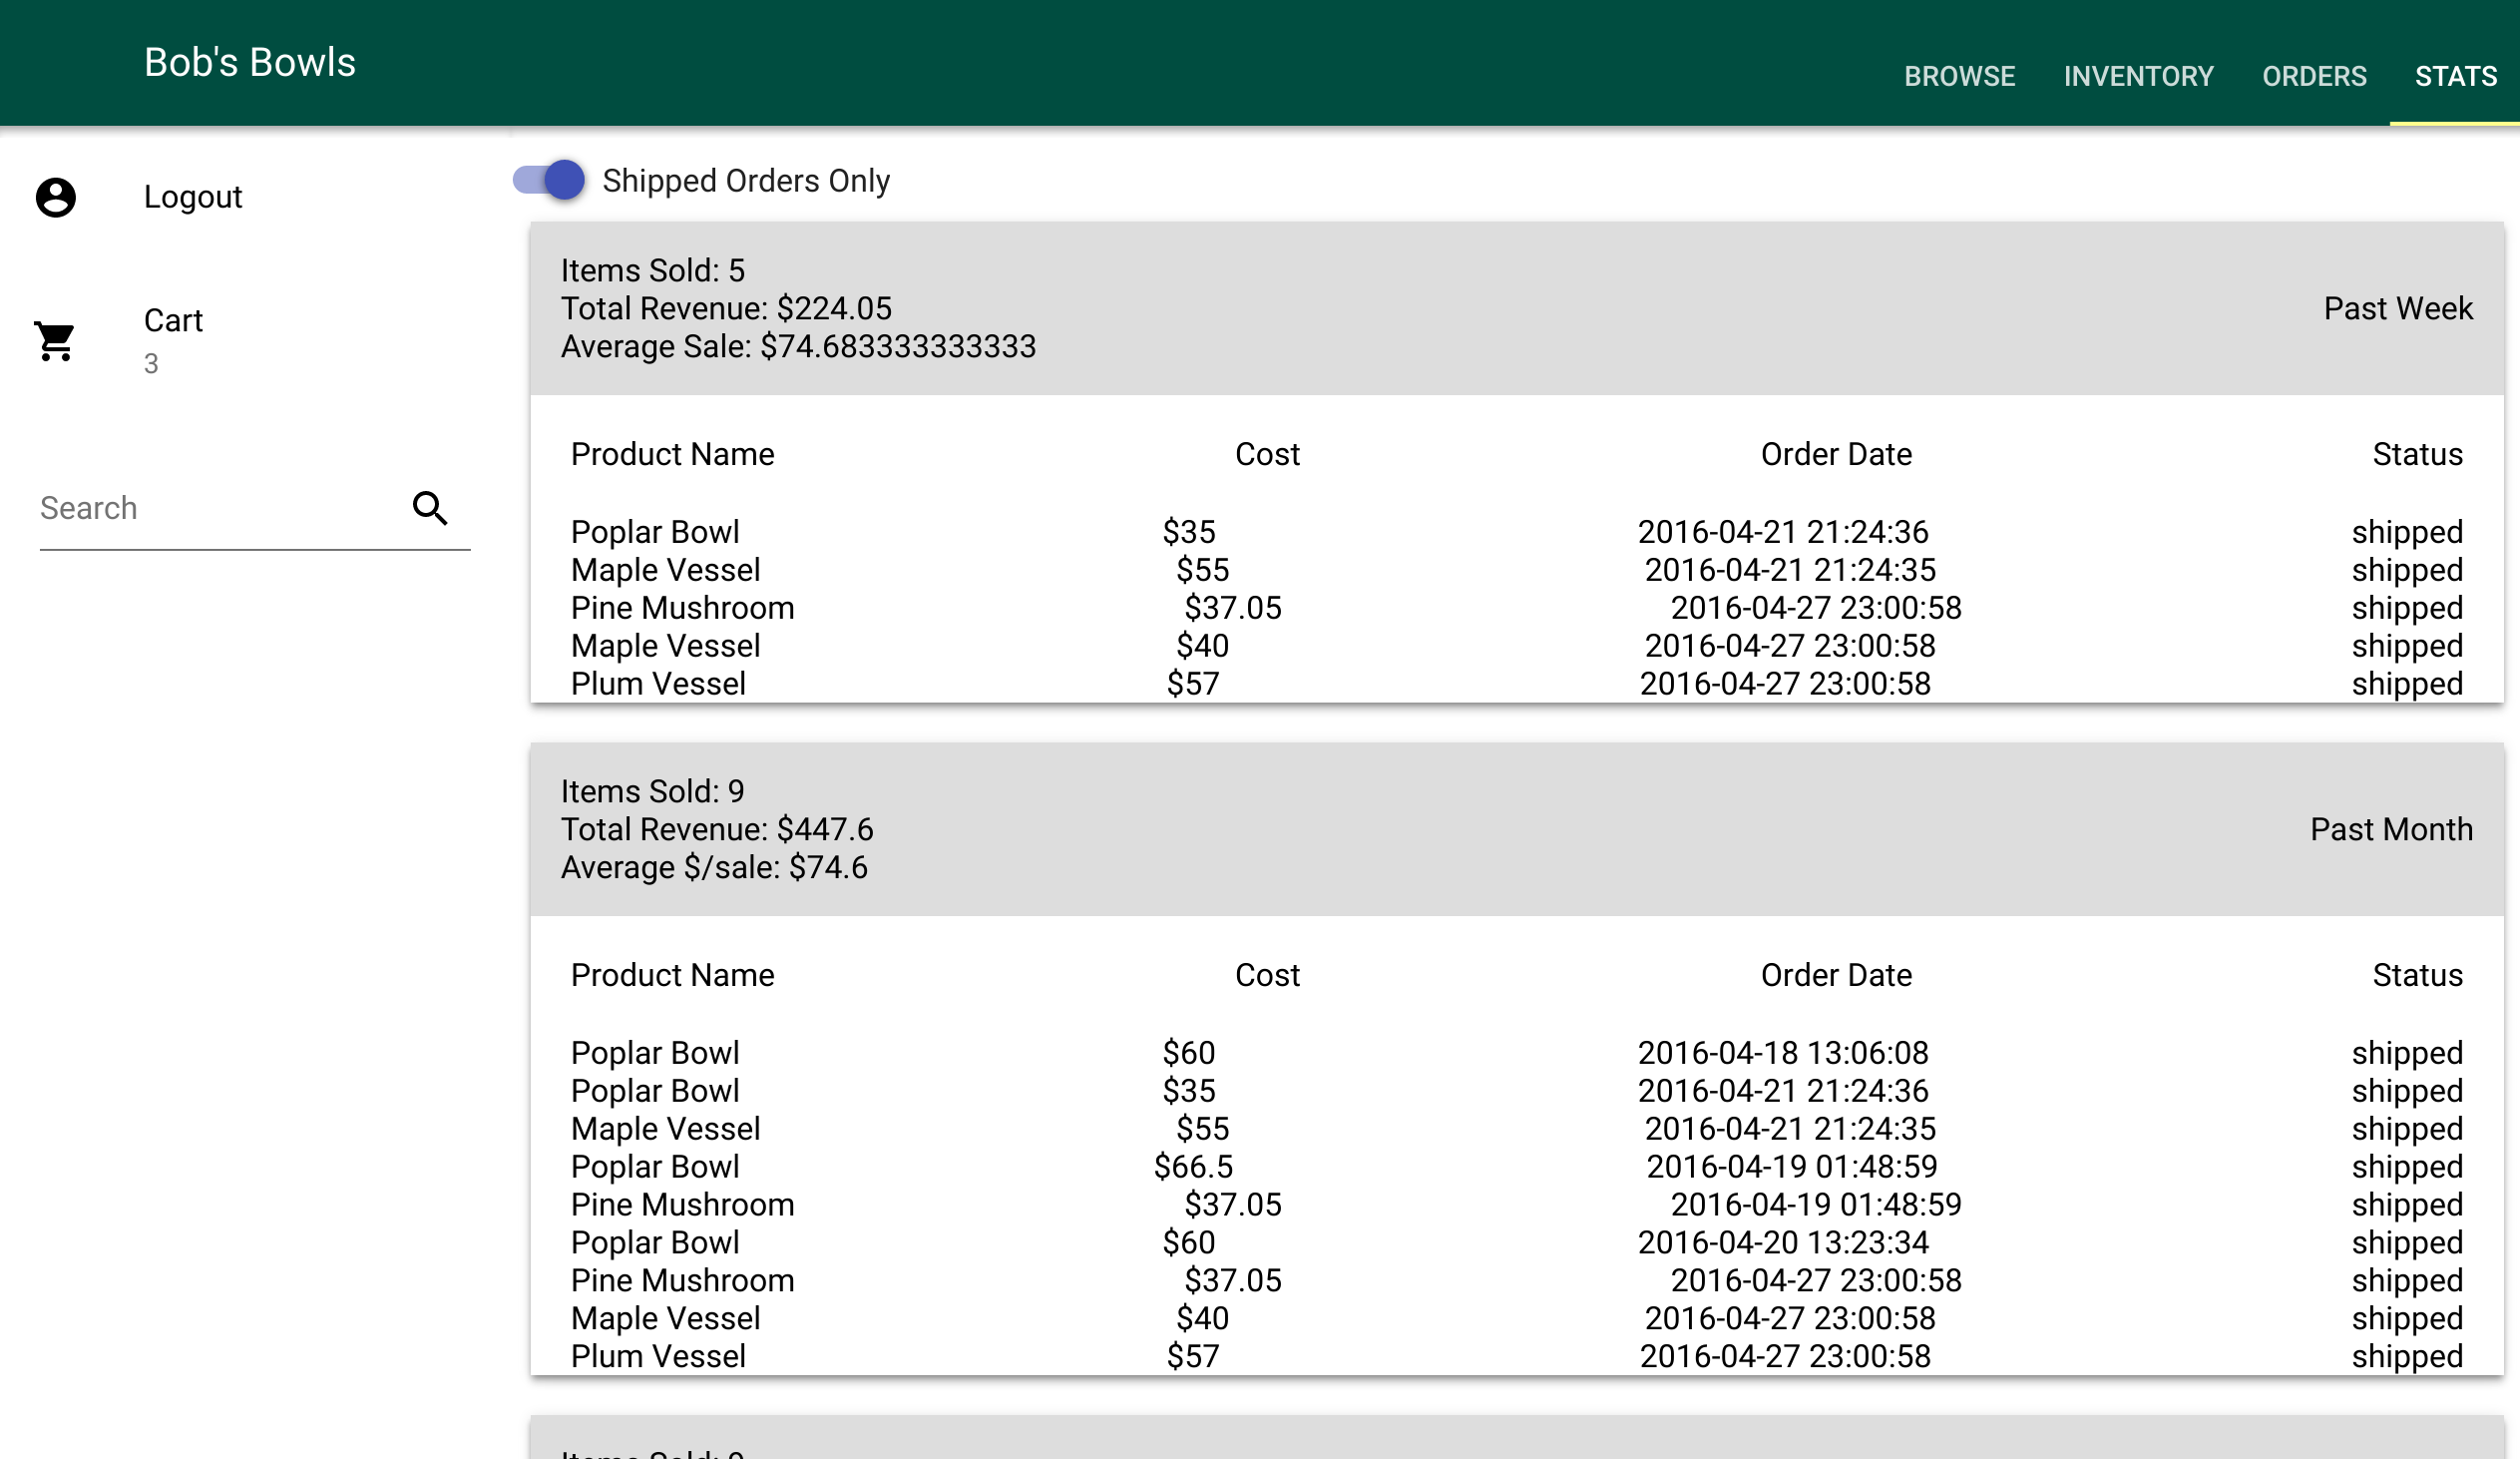
\includegraphics[width=.8\textwidth]{stats}
\caption{The statistics view for managers only.}
\label{cap-stats}
\end{figure}



\section{Testing}
\subsection{Explain what you have tested to make sure your software works correctly}

In testing our database application, we took the assumption that there could be no SQL injection with our front end.  Thus, we only have to handle faulty input, not malicious input.  In testing normal interaction with the database we simulated a moderate amount of commerce traffic in using the application as a customer, staff, and manager user.  

We tested the effectiveness of our trigger statements by trying faulty input (entering negative quantities and discounts greater than 100\% or less than 0\%).  Our triggers caught the faulty input and handled it appropriate by setting the value to something valid.  In the case of discount, it rejects the input and sets back to the prior discount.  On the case of negative quantity, the quantity is set to zero instead.  We’ve used it on multiple to make sure that the updates to inventory and price occur with a refresh or page change in real time.

\subsection{Describe your project experience}

In our experience, the project was mostly a learning experience for SQL and database design.  In contrast it was most a chance to show off some depth of knowledge of website design.  The pre-existing knowledge of programming interactivity and websites proved invaluable for showing off a good database foundation.  The work itself was long but easy to spread out.  Communicating the needs of the different parts of our project was key as interfacing between the two took longer than expected.  The project truly showcased how important it is to balance all the moving parts of a web application.
\begin{thebibliography}{9}
\bibitem{polymer}
Polymer Element Catalog\\
\texttt{https://www.polymer-project.org/1.0/}
\end{thebibliography}
\end{document}

